\chapter{Calorimeter Optimisation Studies}
\label{chap:detopt}

\chapterquote{There, sir! that is the perfection of vessels!}
{Jules Verne, 1828--1905}

\section{Calorimeter Optimisation Studies}
If the future linear collider is to reach it's maximum potential in terms of energy resolution then, optimisation of the detector will be essential.  The energy resolution in the particle flow paradigm is dependant upon several detector components.  The momentum of charged particles arises from the shape of the tracks deposited within the detector while the energy of uncharged particles arise from calorimetric measurements.  Application of sophisticated pattern recognition algorithms allows the particle type to be inferred for the charged particles.  In tern this allows for the conversion of the track momentum into an energy measure for the charged particles.  The particle identification algorithms use the topological information acquired from the calorimetric energy deposited to infer particle type for a subset of charged particles.  

The calorimetric energy deposits are therefore used in a twofold manner: (i) as energy measurements for neutral particles and (ii) as input for particle identification algorithms.  There is potential for significant gains to be made in physics performance by optimising the calorimeters due to their dominant role in energy measurements.  In this chapter the optimisation of the calorimeters is considered.  Parameters such as the longitudinal granularity, transverse granularity and material choices for the calorimeters are considered.  

This chapter concludes with an optimisation of several global parameters for the detector.  These parameters are not calorimeter specific, but the optimisation procedure developed for the calorimeters is appropriate to use.  These parameters relate to the global detector size and the magnetic field applied throughout solenoid in the detector.

\section{Metric}

\section{Simulation and Reconstruction}

\section{Calibration}

\section{Nominal Detector Performance}
The energy resolution for single photon events as a function of photon energy, for the nominal ILD detector, is shown in figure \ref{fig:ecalnominalres}.  The nominal jet energy resolution can be found in section BLAH.

\begin{figure}
\centering
\subfloat[Silicon active material, $5 \times 5 \text{mm}^{2}$ ECal transverse granularity.]{\label{fig:ecalsinominalres}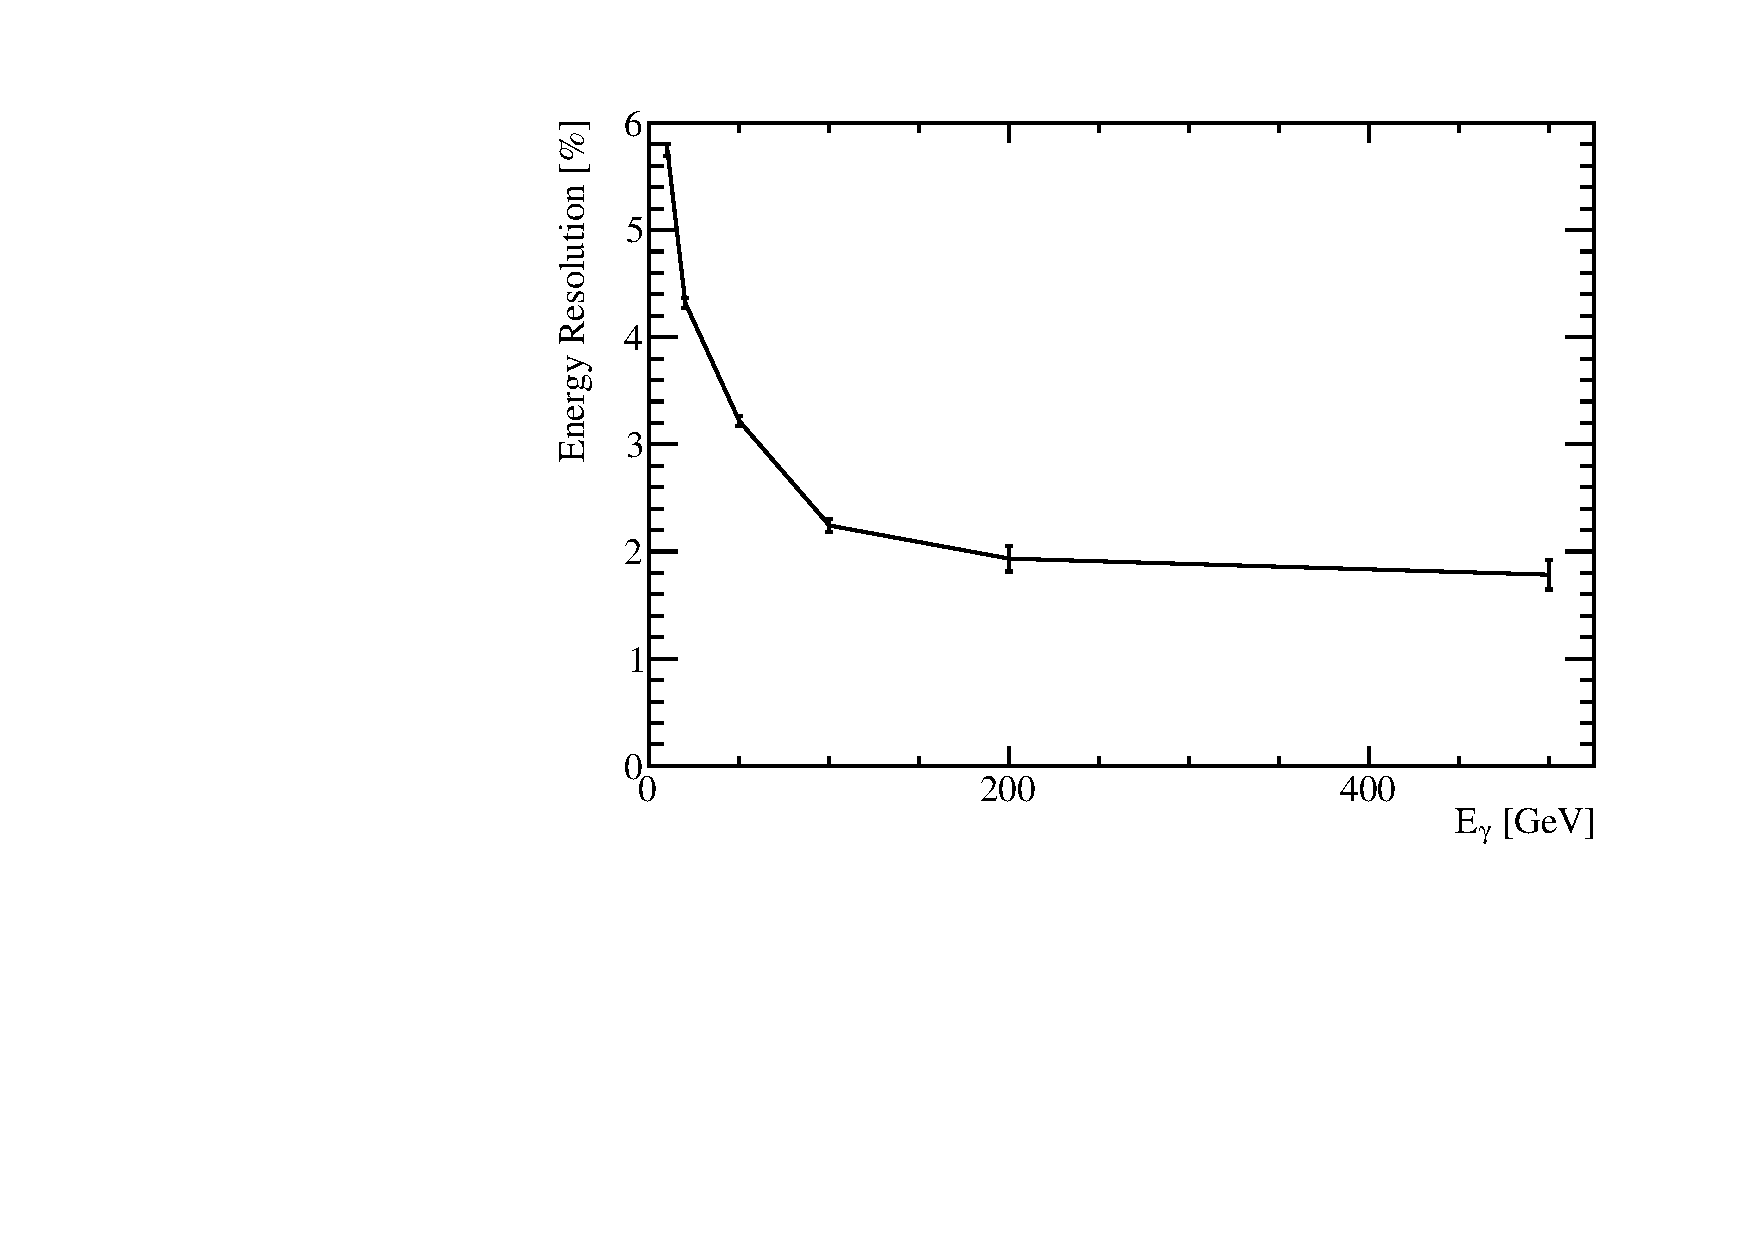
\includegraphics[width=0.5\textwidth]{OptimisationStudies/Plots/EnergyResolution/ER_vs_EGamma_SiliconECal.pdf}}
\subfloat[Scintillator active material, $5 \times 5 \text{mm}^{2}$ ECal transverse granularity.]{\label{fig:ecalscnominalres}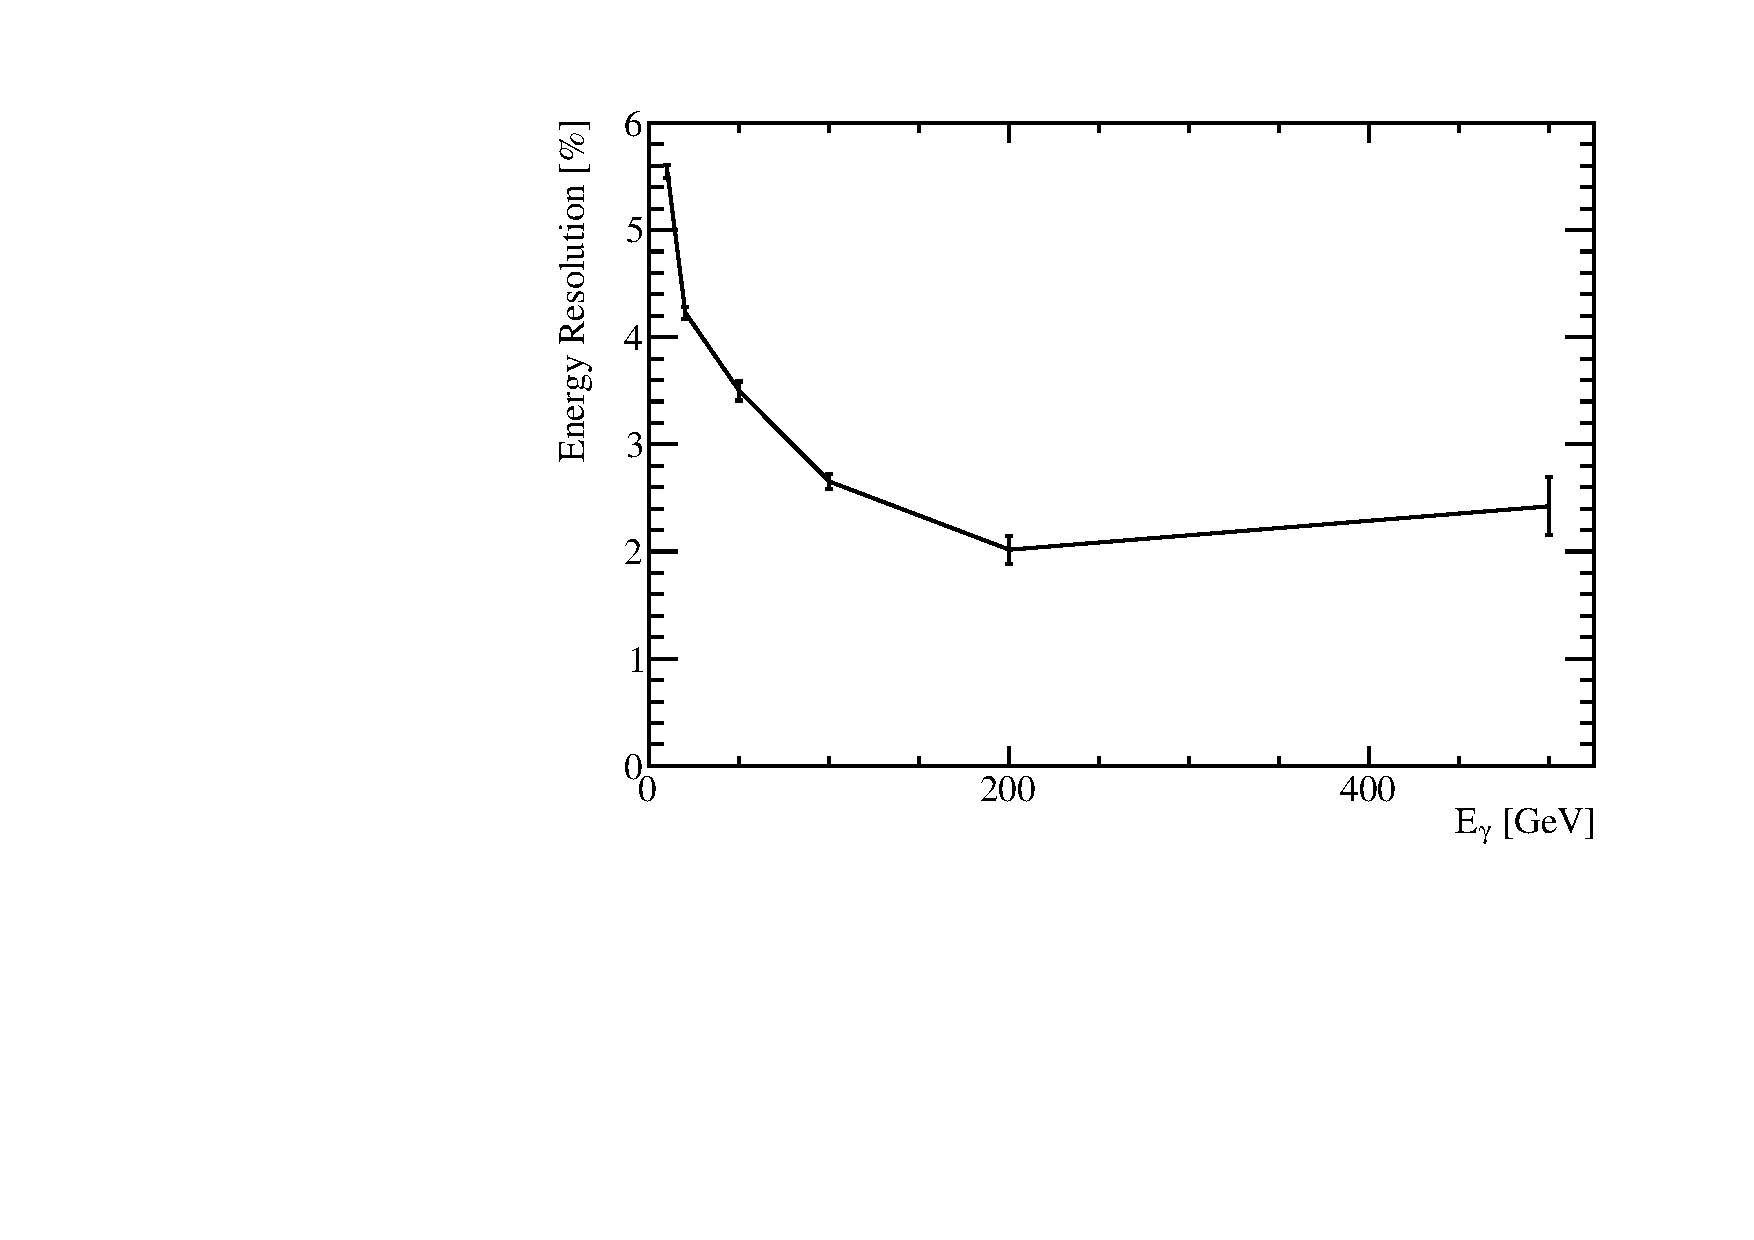
\includegraphics[width=0.5\textwidth]{OptimisationStudies/Plots/EnergyResolution/ER_vs_EGamma_ScintillatorECal.pdf}}
\caption[Energy resolution as a function of photon energy for the nominal ILD detector for both the silicon and scintillator options.]{Energy resolution as a function of photon energy for the nominal ILD detector for both the silicon and scintillator options.}
\label{fig:ecalnominalres}
\end{figure}

\section{Electromagnetic Calorimeter Optimisation}
\label{sec:ecal}
The ECal primarily measures the energy deposits of electromagnetic showers.  The default ILD detector model, summarised in table \ref{table:defaultildecal}, contains 24 radiation lengths ($\text{X}_{0}$, which acts to confine all but the highest energy electromagnetic showers within it.  The longitudinal structure of this default model is 29 readout layers, consisting of pairs of active and absorber material, and one presampling layer, which exists to encourage shower development.  Increasing the thickness of the absorber material part way into the detector reduces the number of readout channels and cost of the overall calorimeter while retaining a high sampling rate at the start of particle showers, which is crucial for the pattern recognition aspect of particle flow calorimetry.  

\begin{table}[h!]
\centering
\begin{tabular}{ l l}
\hline
Parameter & Default Value \\
\hline
Transverse Granularity & $5 \times 5 \text{mm}^{2}$ square cells \\
Longitudinal Granularity & 29 Readout Layers, 1 Presampling Layers \\
Active Material Choice & Silicon or Scintillator  \\
Active Material Thickness & 0.5 mm (Silicon) or 2 mm (Scintillator)  \\
Absorber Material Choice & Tungsten \\
Absorber Material Thickness & 20 Layers of 2.1 mm followed by 9 Layers of 4.2 mm \\
\hline
\end{tabular}
\caption{Cross section for selected processes for given value of $\alpha_{4}$ and $\alpha_{5}$ at 1.4 TeV.}
\label{table:defaultildecal}
\end{table}

The parameters being optimised in this study are:
\begin{itemize}
\item Transverse granularity or cell size.  This is a vital aspect of the detector in the particle flow paradigm as smaller cell sizes give greater potential for being able to separate energy deposits from charged and neutral particles.  This transverse granularity should have little to no effect on the intrinsic energy resolution of the detector.  
\item Longitudinal granularity or cell depth.  This parameter dictates the intrinsic energy resolution of the detector as smaller cell depths mean more sampling is done of the particle shower and so, due to the Poissonian statistics governing the measurement of particle showers, the better the resolution.
\item Active material choice.  This is a choice between silicon or scintillator.  As well as providing different intrinsic energy resolutions the readout mechanics of these two options are significantly different.  There is no clear prior knowledge as to which should provide better performance. 
\end{itemize}

\subsection{ECal Transverse Granularity}
For this study a number of different detector models were considered where the transverse granularity in the ECal had been varied about the nominal value of $5 \times 5 \text{mm}^{2}$ square cells.  The granularities considered were $3 \times 3 \text{mm}^{2}$, $5 \times 5 \text{mm}^{2}$, $7 \times 7 \text{mm}^{2}$, $10 \times 10 \text{mm}^{2}$, $15 \times 15 \text{mm}^{2}$ and $20 \times 20 \text{mm}^{2}$ square cells for both the silicon and scintillator active material options.  The jet energy resolution for these detector models as a function of transverse granularity in the ECal is shown in figure \ref{fig:ecalcellsize}.

\begin{figure}
\centering
\subfloat[Silicon active material.]{\label{fig:ecalsicellsize}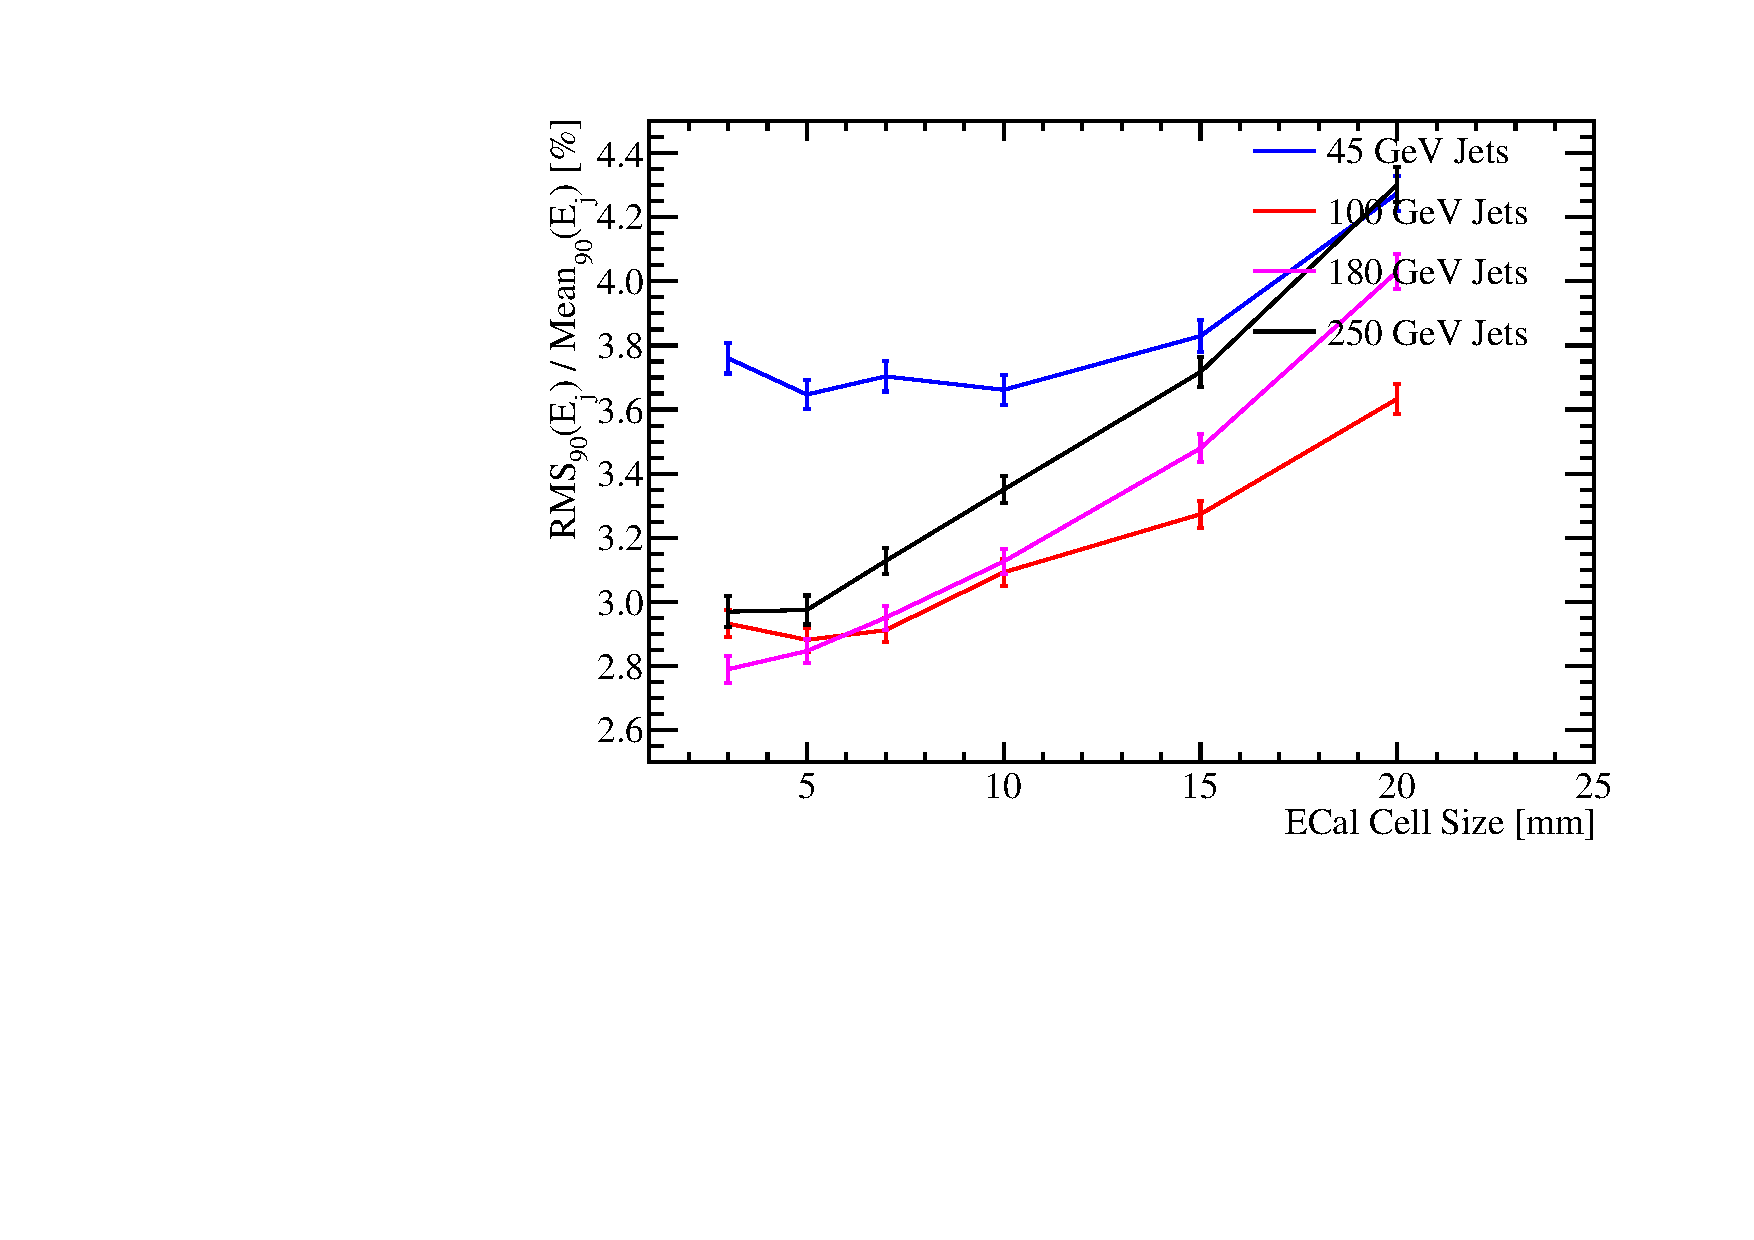
\includegraphics[width=0.5\textwidth]{OptimisationStudies/Plots/JetEnergyResolutions/JER_vs_SiliconECalCellSize.pdf}}
\subfloat[Scintillator active material.]{\label{fig:ecalsccellsize}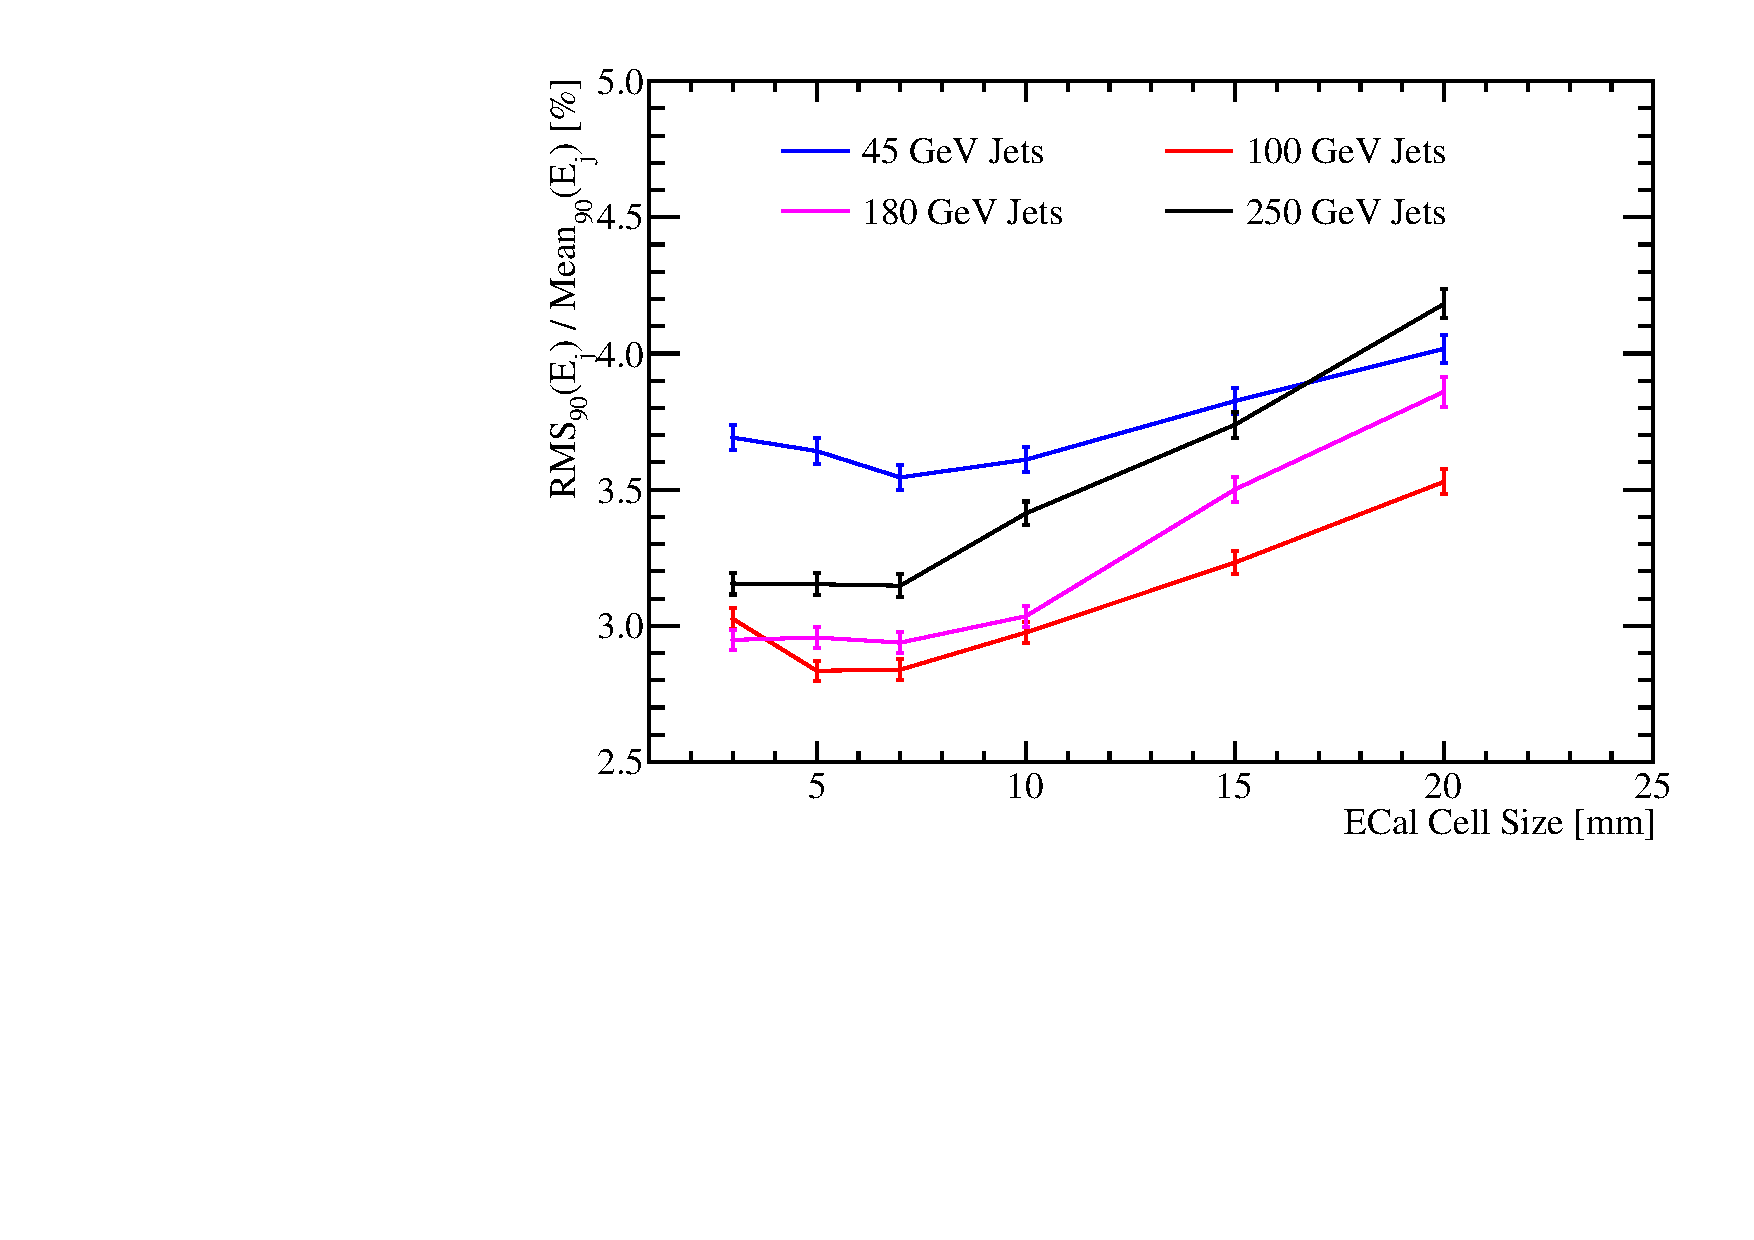
\includegraphics[width=0.5\textwidth]{OptimisationStudies/Plots/JetEnergyResolutions/JER_vs_ScintillatorECalCellSize.pdf}} \hfill
\caption[Jet energy resolution as a function of ECal cell size.]{Jet energy resolution as a function of ECal cell size for the silicon and scintillator ECal options.}
\label{fig:ecalcellsize}
\end{figure}

The jet energy resolution was found to improve with decreasing cell size.  This is expected as smaller cell size lead to better separation of energy deposits from neutral and charged particle showers.  

\begin{figure}
\centering
\subfloat[Silicon active material, 45 GeV Jets.]{\label{fig:ecalsicellsize45break}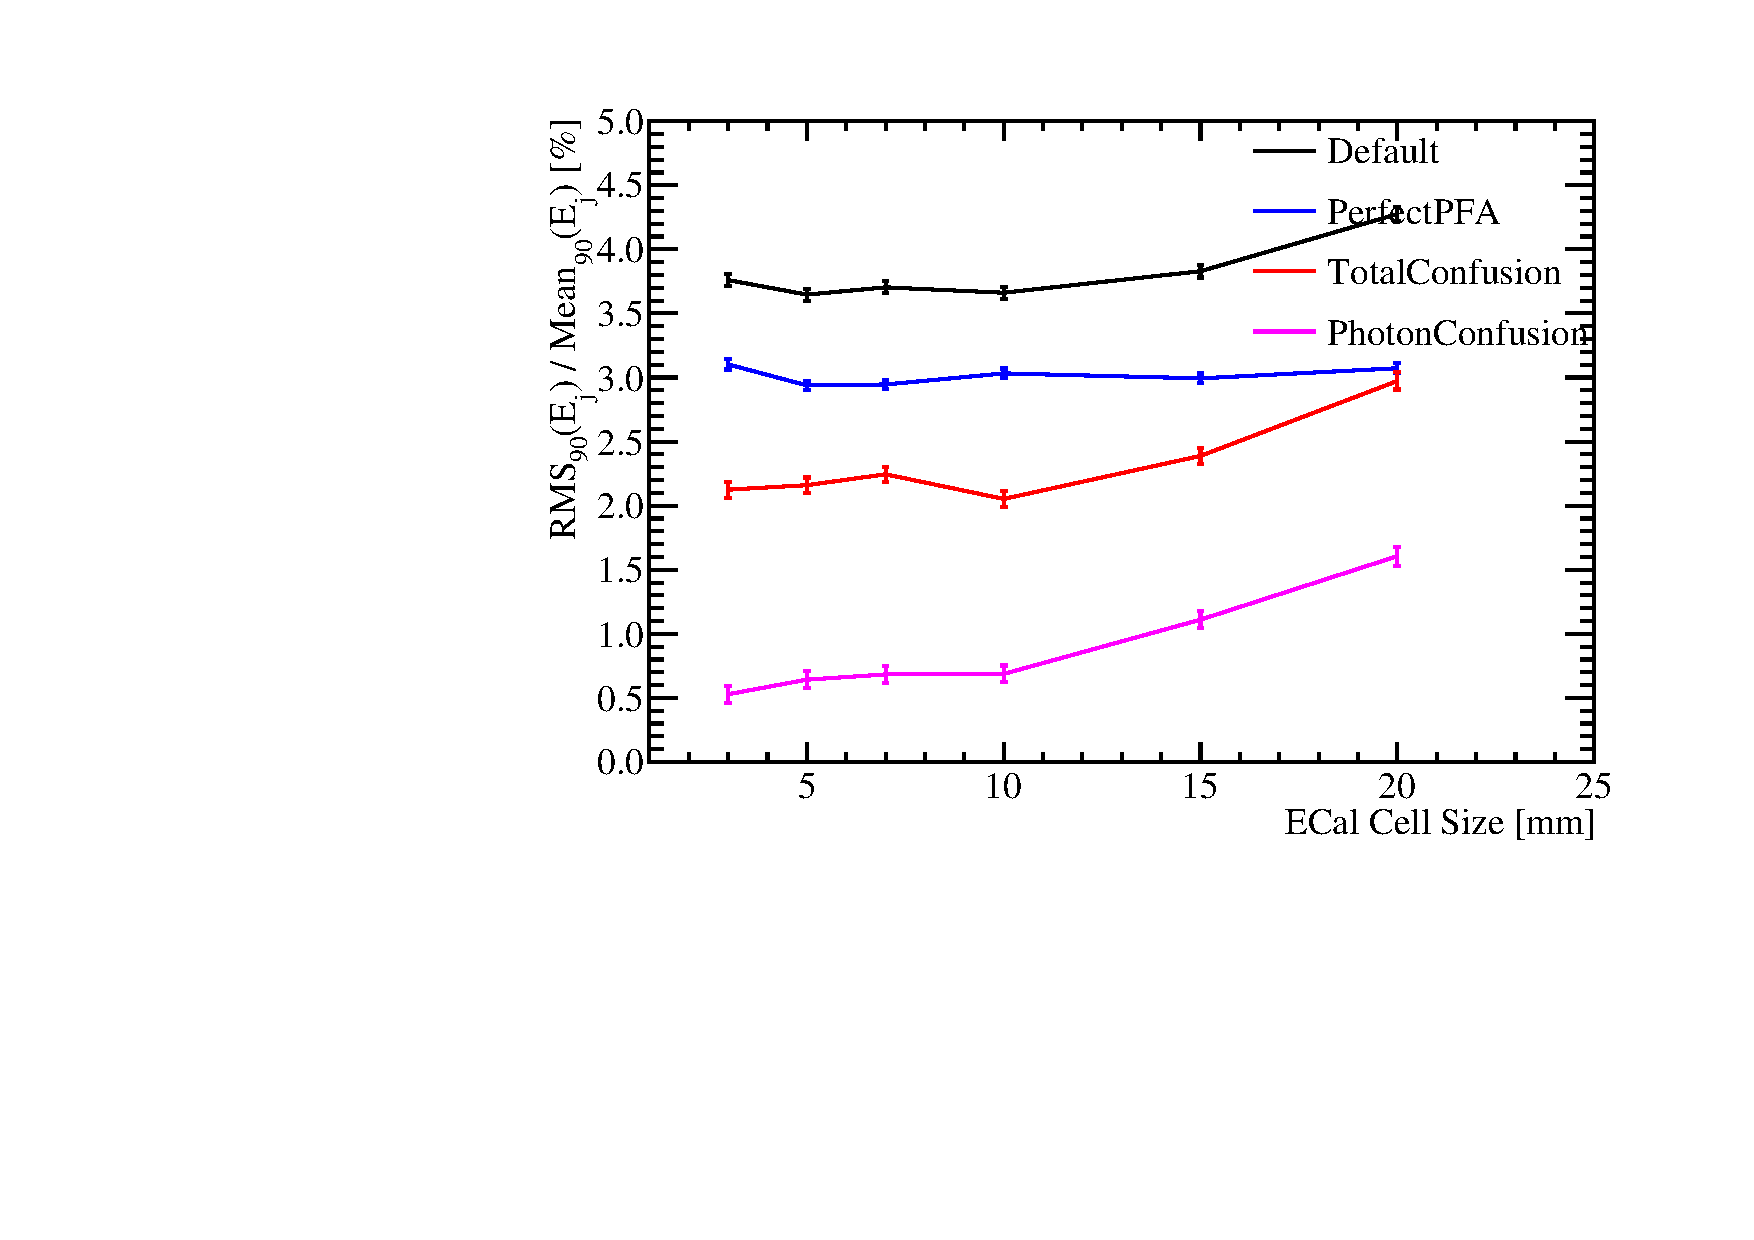
\includegraphics[width=0.5\textwidth]{OptimisationStudies/Plots/JetEnergyResolutions/JER_vs_SiliconECalCellSize_91GeV_DiJet_Breakdown.pdf}}
\subfloat[Scintillator active material, 45 GeV Jets.]{\label{fig:ecalsccellsize45break}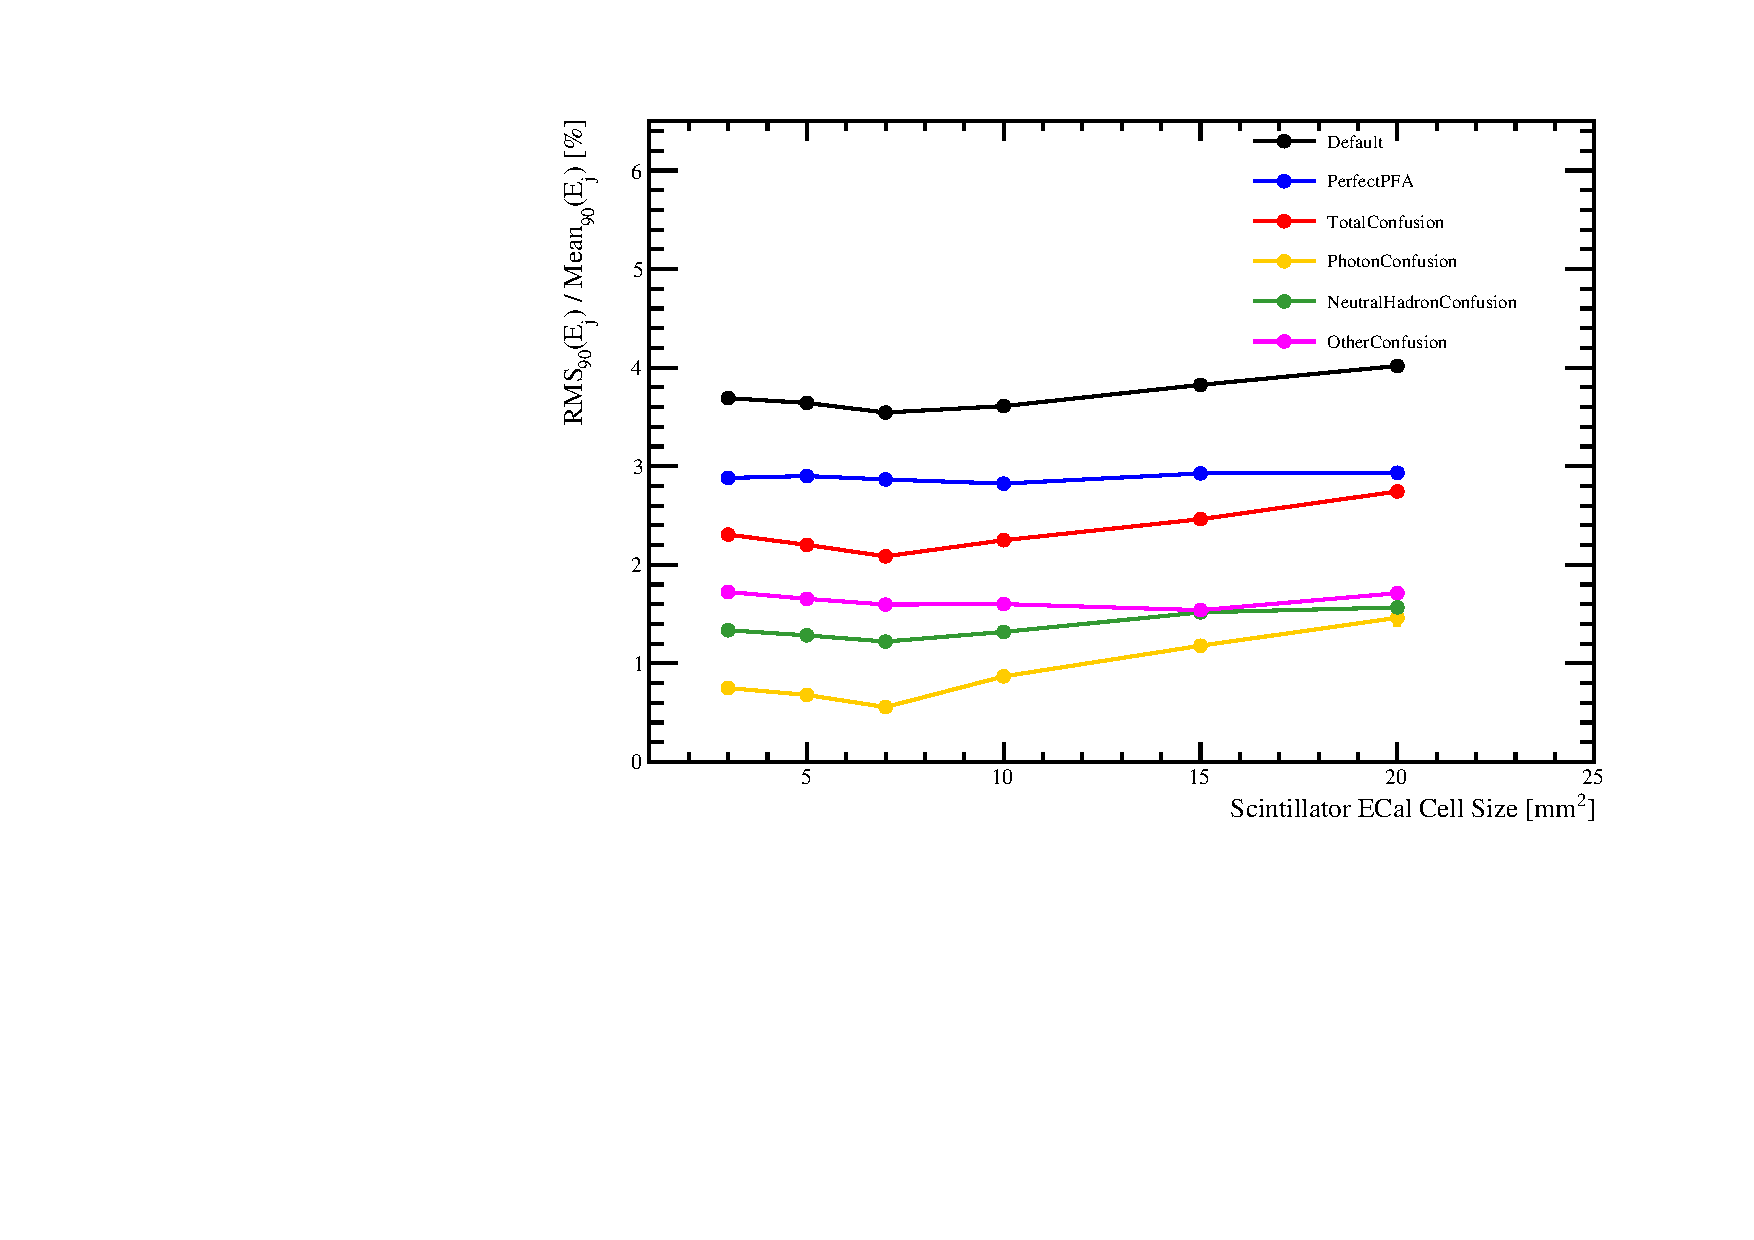
\includegraphics[width=0.5\textwidth]{OptimisationStudies/Plots/JetEnergyResolutions/JER_vs_ScintillatorECalCellSize_91GeV_DiJet_Breakdown.pdf}} \hfill
\subfloat[Silicon active material, 250 GeV Jets.]{\label{fig:ecalsicellsize250break}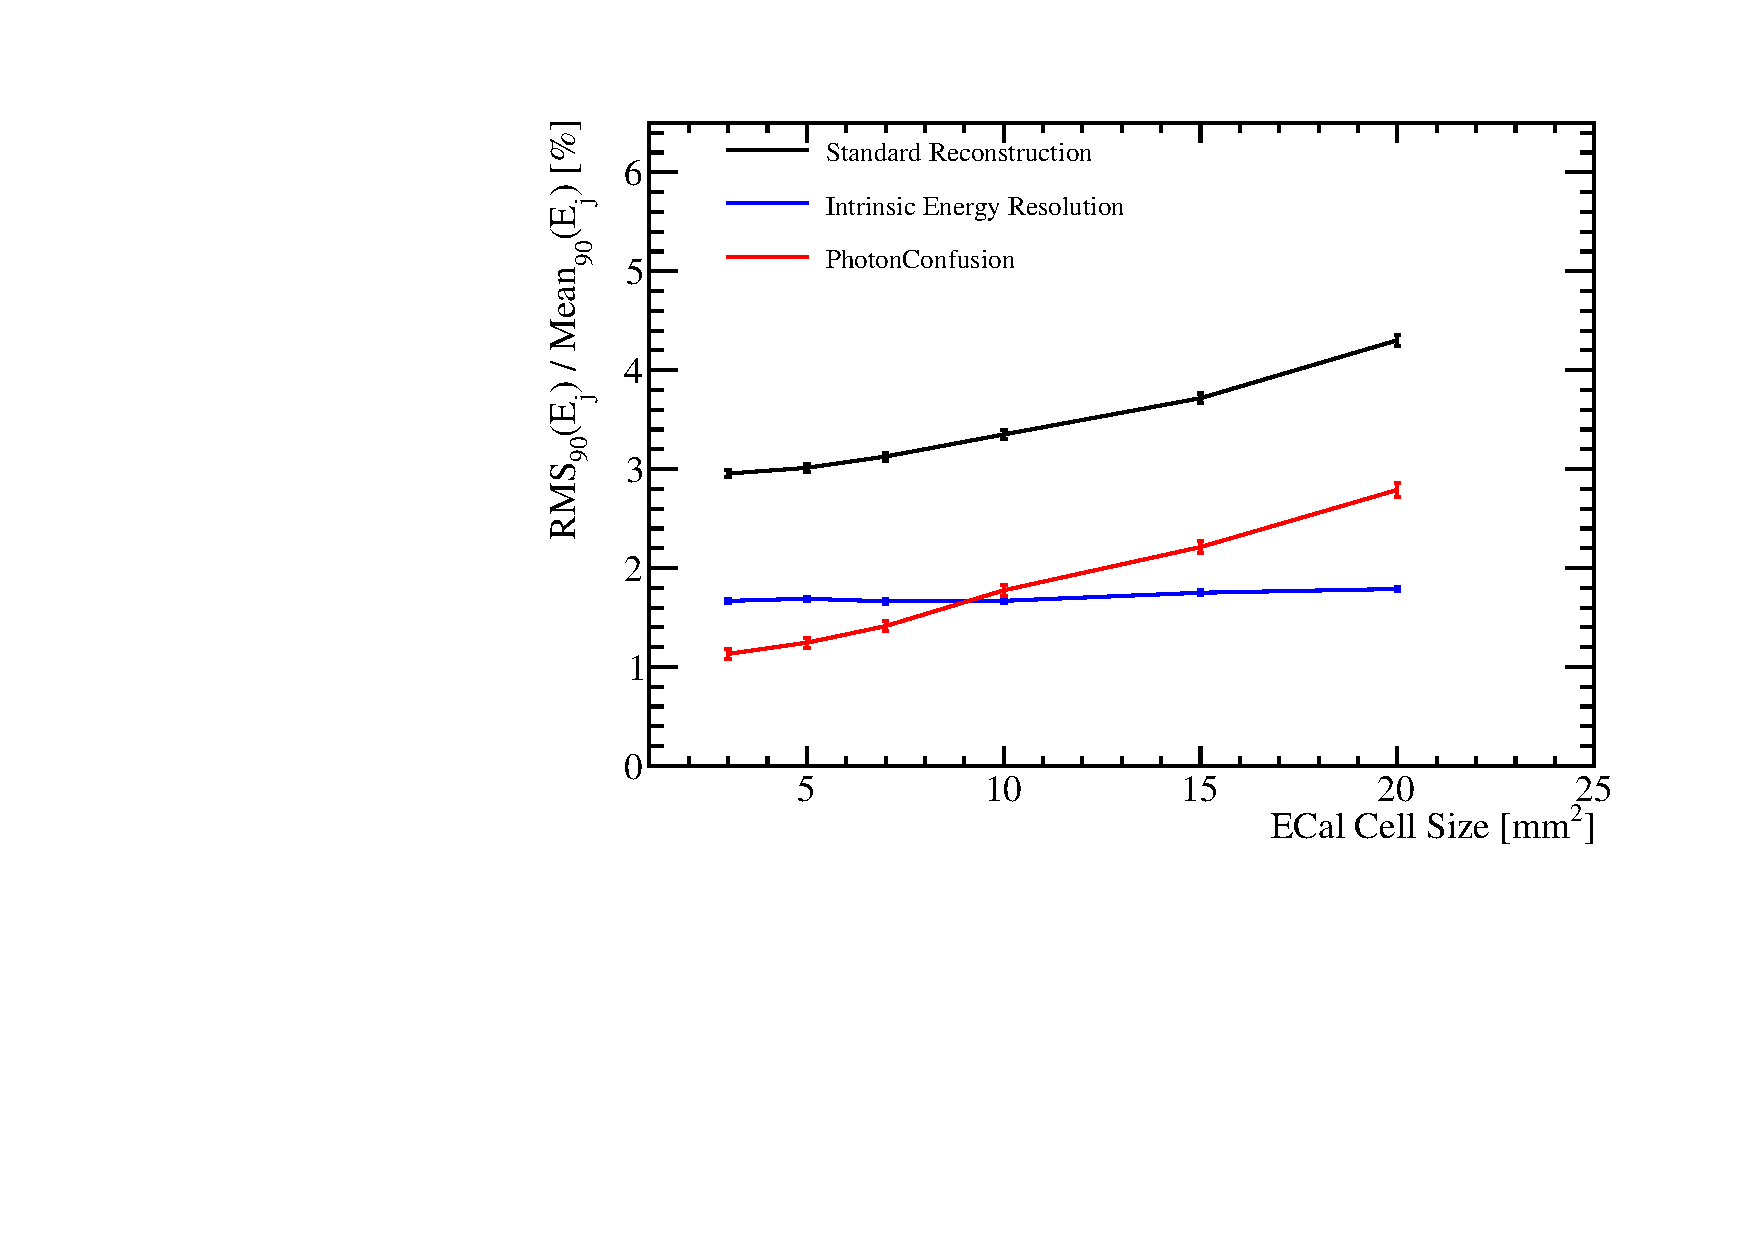
\includegraphics[width=0.5\textwidth]{OptimisationStudies/Plots/JetEnergyResolutions/JER_vs_SiliconECalCellSize_500GeV_DiJet_Breakdown.pdf}}
\subfloat[Scintillator active material, 250 GeV Jets.]{\label{fig:ecalsccellsize250break}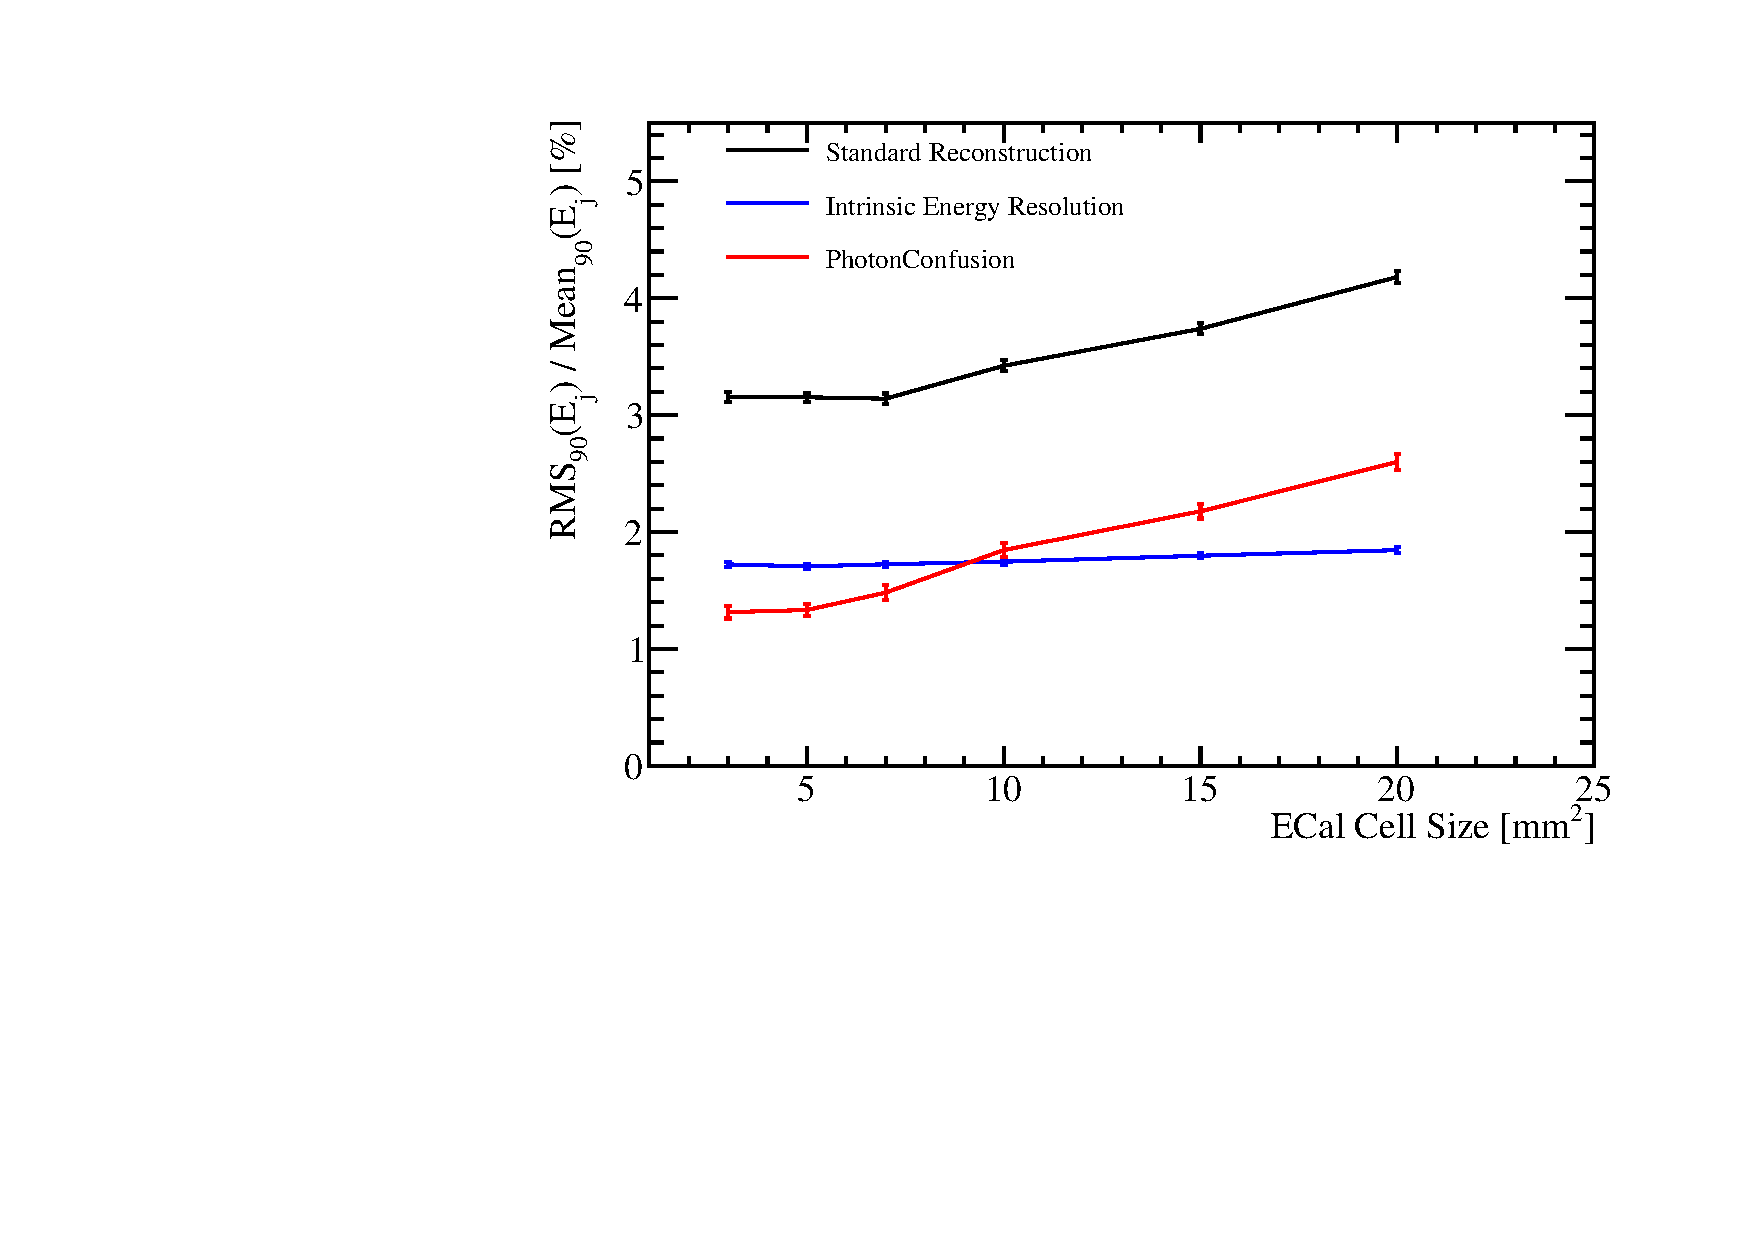
\includegraphics[width=0.5\textwidth]{OptimisationStudies/Plots/JetEnergyResolutions/JER_vs_ScintillatorECalCellSize_500GeV_DiJet_Breakdown.pdf}}
\caption[Jet energy resolution breakdown as a function of ECal transverse granularity for 45 and 250 GeV jets.  Results are given for both the silicon and scintillator ECal options.]{Jet energy resolution breakdown as a function of ECal transverse granularity for 45 and 250 GeV jets.  Results are given for both the silicon and scintillator ECal options.}
\label{fig:ecalcellsize}
\end{figure}

By examining the breakdown of the jet energy resolution into intrinsic resolution and confusion terms, as explained in chapter BLAH, it is possible to conclude that the dominant factor affecting the jet energy resolution when the transverse granularity of the ECal is varied is the confusion arising from photon energy deposits.  Examples of jet energy resolution breakdowns are shown for 45 and 250 GeV jets for both the silicon and scintillator ECal options in figure \ref{fig:ecalcellsize}.  As expected in the intrinsic energy resolution does not change significantly with the transverse granularity.  

\begin{figure}
\centering
%\subfloat[Silicon active material, 10 GeV $\gamma$.]{\label{fig:ecalsicellsize10gamma}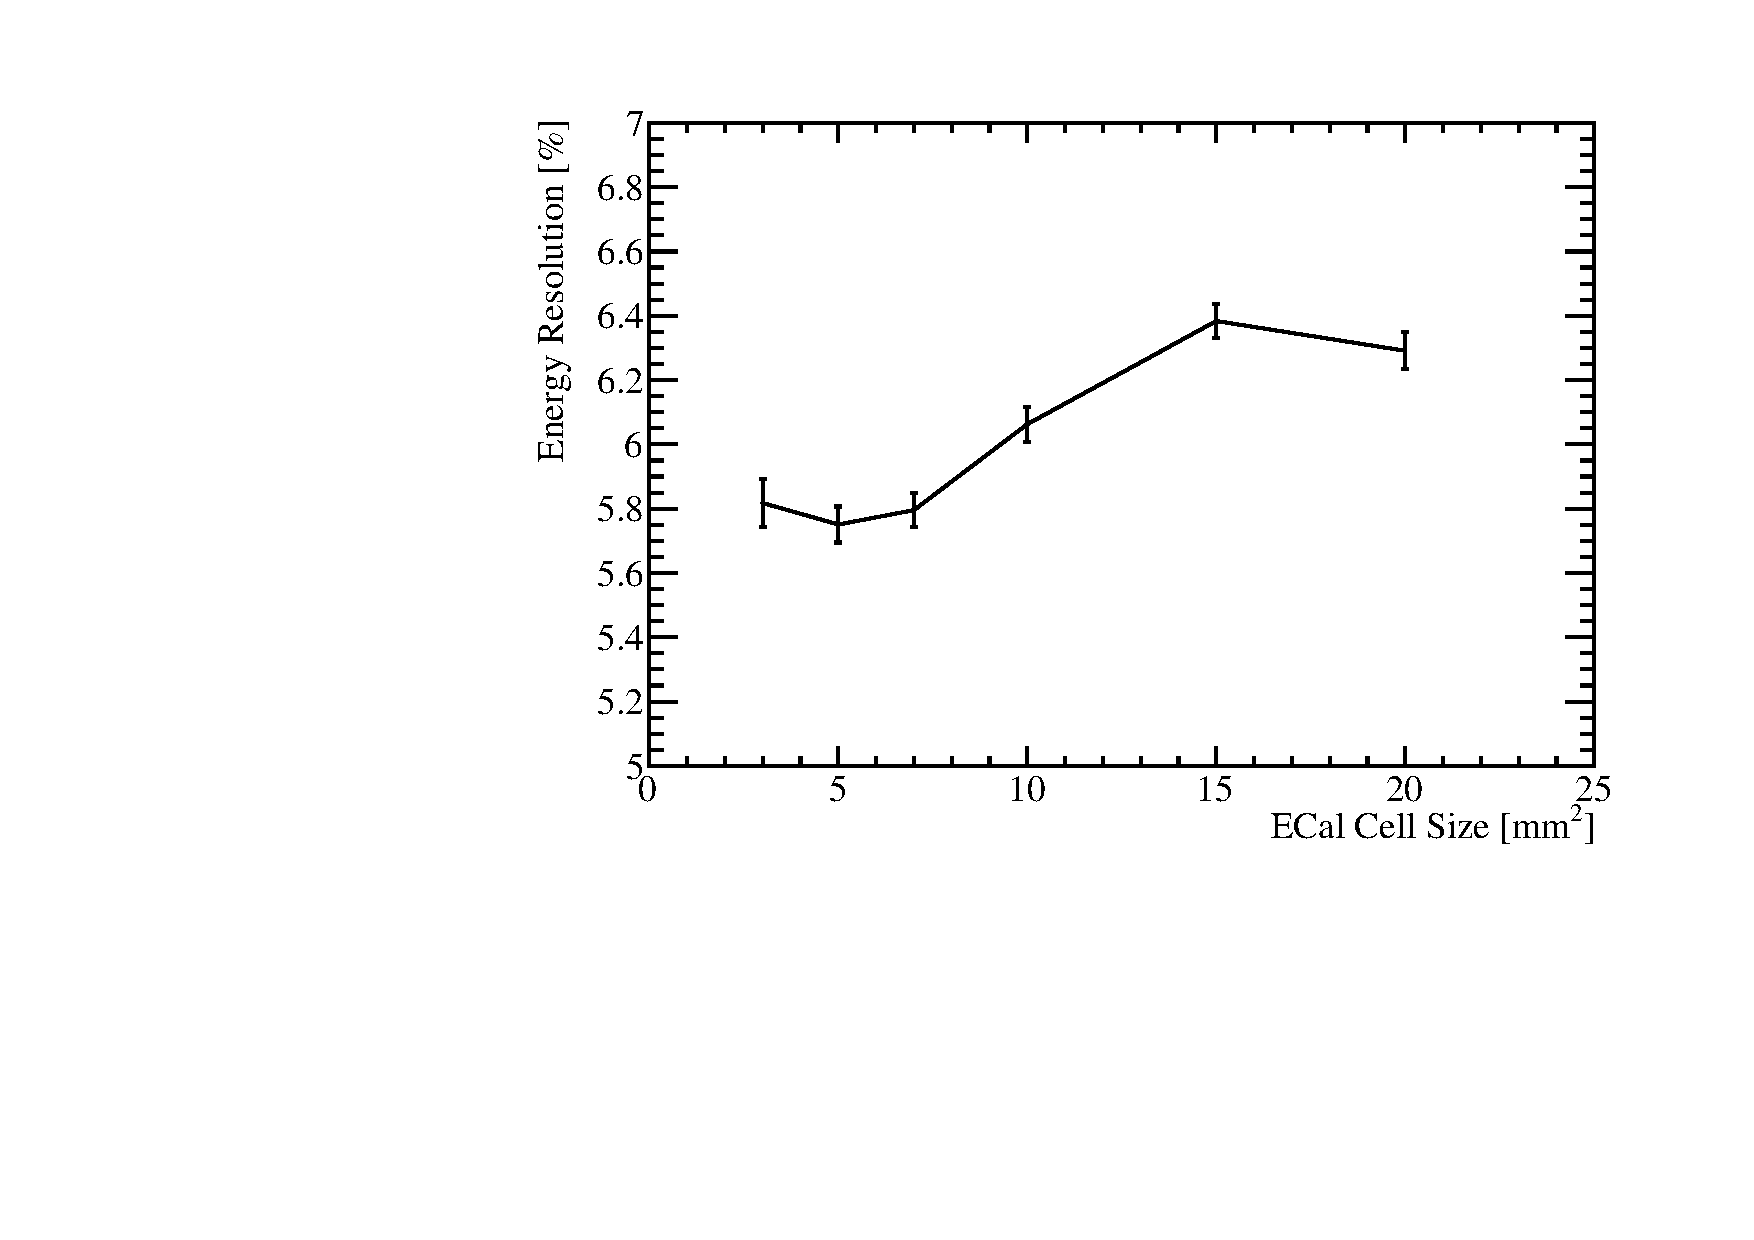
\includegraphics[width=0.5\textwidth]{OptimisationStudies/Plots/EnergyResolution/SiECal10GeVPhotonResVsCellSize.pdf}} // Bit too messy to draw good conclusions
%\subfloat[Scintillator active material, 10 GeV $\gamma$.]{\label{fig:ecalsccellsize10gamma}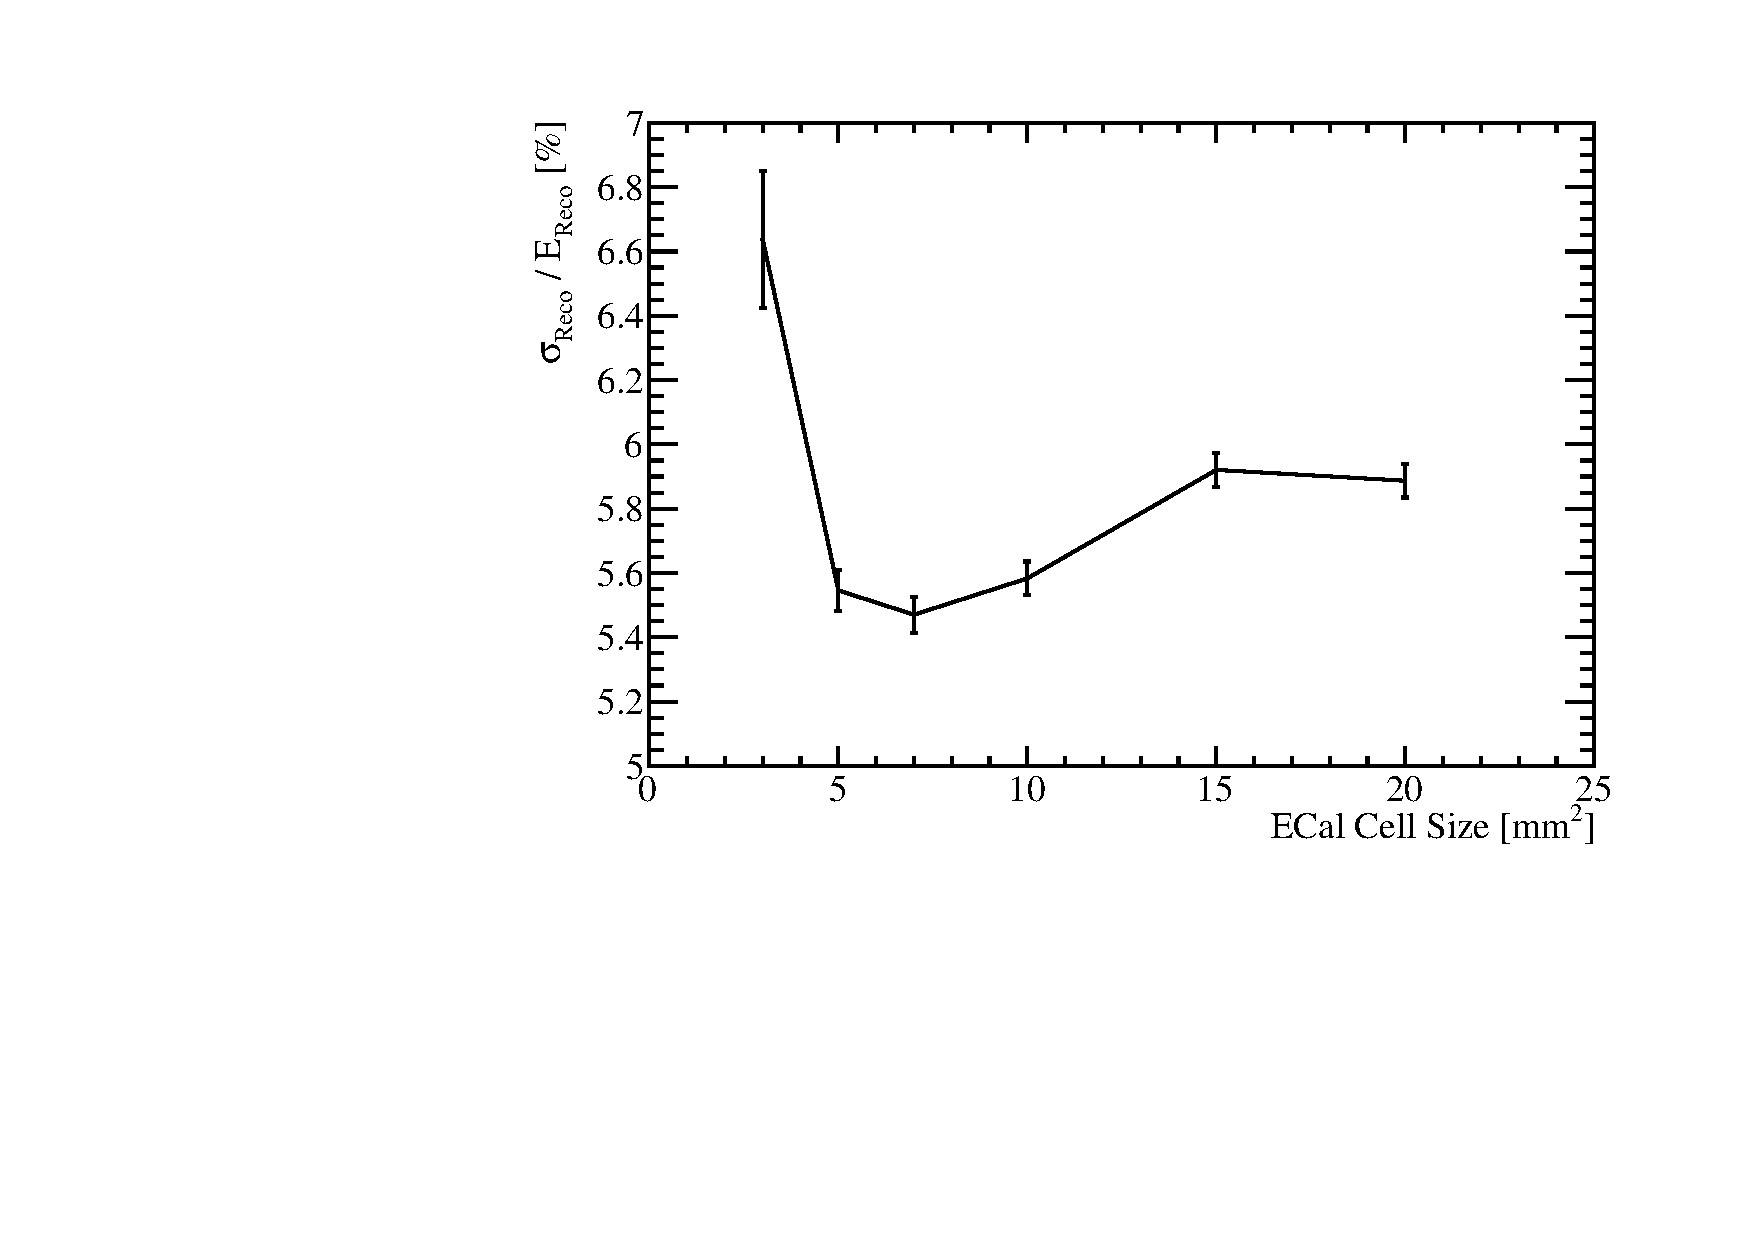
\includegraphics[width=0.5\textwidth]{OptimisationStudies/Plots/EnergyResolution/ScECal10GeVPhotonResVsCellSize.pdf}} \hfil // Bit too messy to draw good conclusions
\subfloat[Silicon active material, 100 GeV $\gamma$.]{\label{fig:ecalsicellsize100gamma}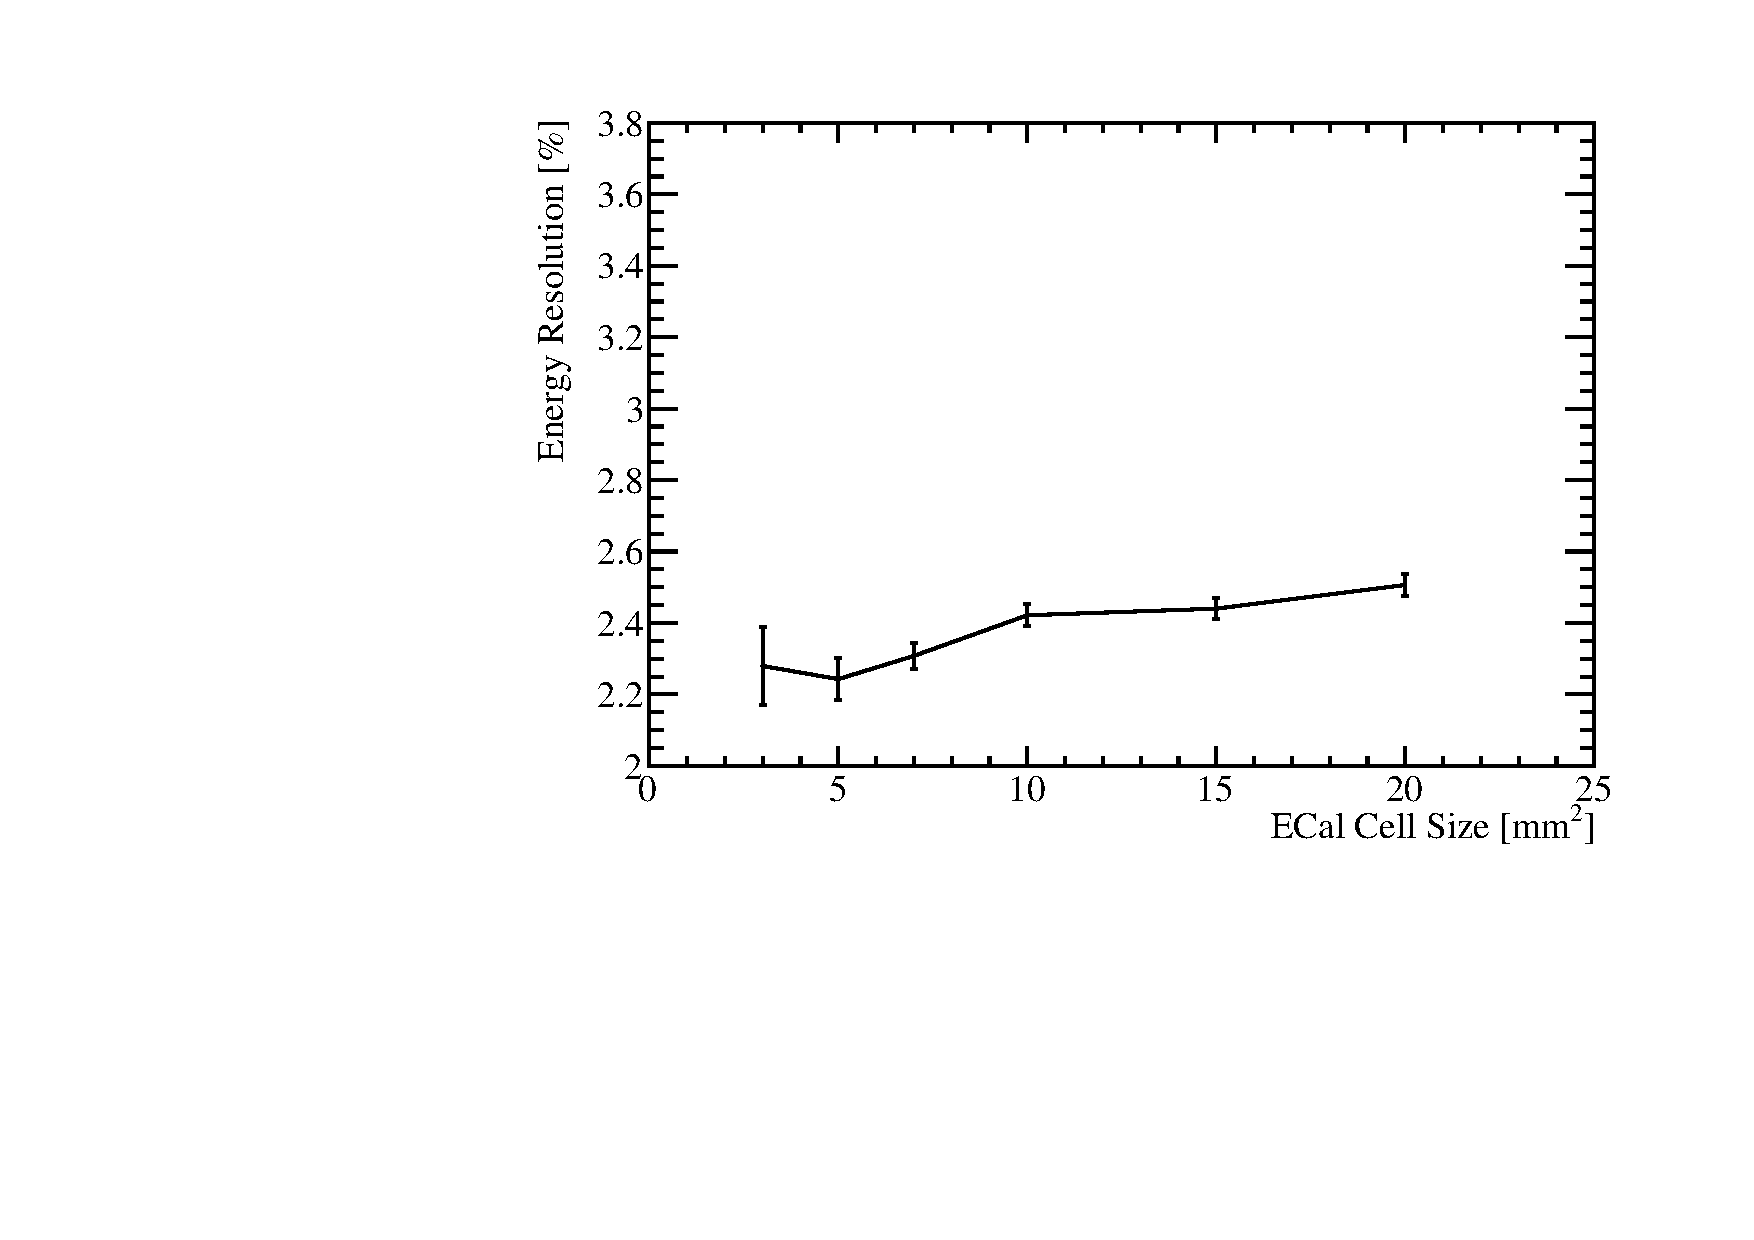
\includegraphics[width=0.5\textwidth]{OptimisationStudies/Plots/EnergyResolution/SiECal100GeVPhotonResVsCellSize.pdf}}
\subfloat[Scintillator active material, 100 GeV $\gamma$.]{\label{fig:ecalsccellsize100gamma}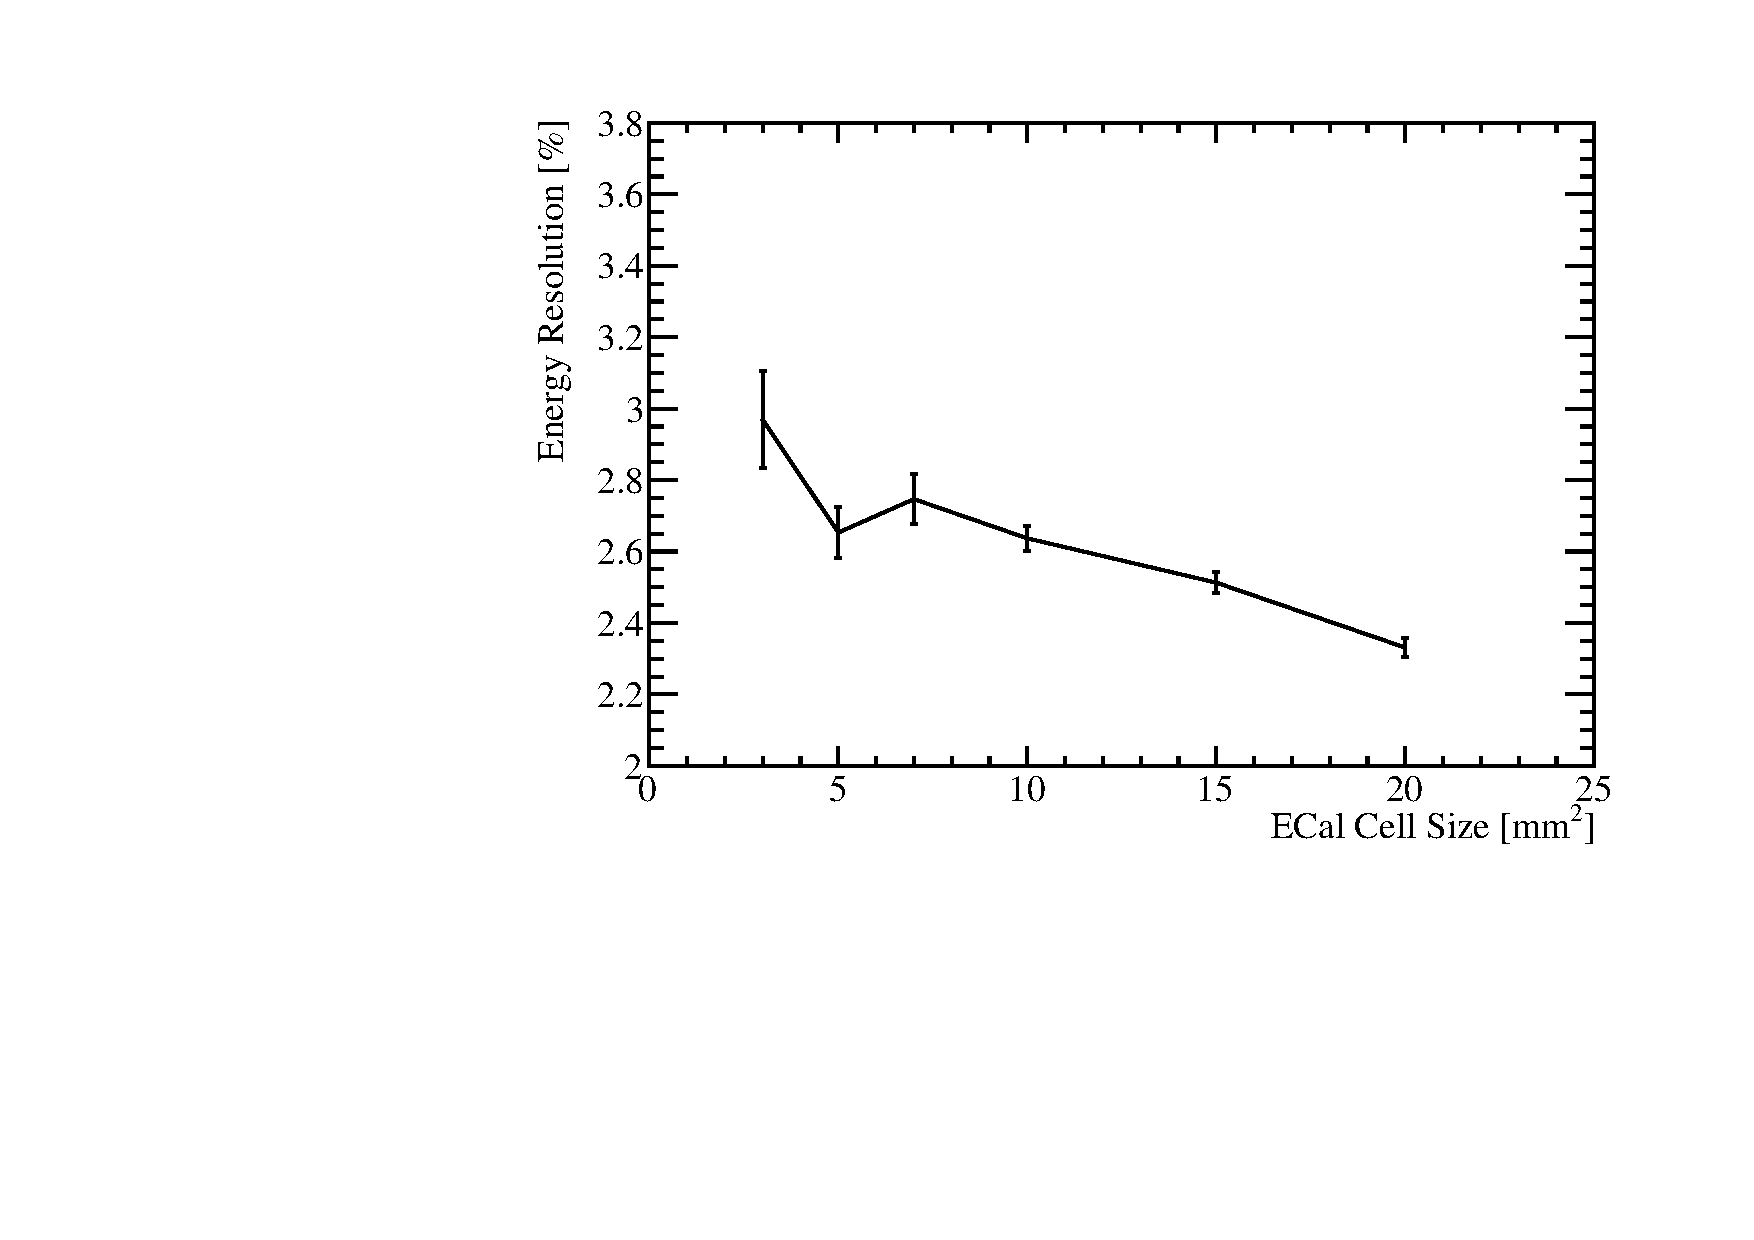
\includegraphics[width=0.5\textwidth]{OptimisationStudies/Plots/EnergyResolution/ScECal100GeVPhotonResVsCellSize.pdf}}
\caption[Energy resolution as a function of ECal transverse granularity for 100 GeV photons.  Results are given for both the silicon and scintillator ECal options.]{Energy resolution as a function of ECal transverse granularity for 100 GeV photons.  Results are given for both the silicon and scintillator ECal options.}
\label{fig:ecalcellsizegamma}
\end{figure}

A more targeted test of the intrinsic energy resolution of the ECal is presented in figure \ref{fig:ecalcellsizegamma}, which examines the energy resolution of single photon samples at 100 GeV.  For the silicon option the intrinsic energy resolution was found to not vary significantly across the transverse granularities under consideration, however, there is a degradation in energy resolution with increasing cell size for the scintillator option.  This originates from an inactive region of material in the simulation that represents the multi pixel photon counter (MPPC).  The MPPC occupies a fixed area of the cell irrespective of cell size and so fractionally the "dead" region of the cell increases as cell size is reduced (cite this somehow).  These trends will be present in the jet energy resolution studies, however, as only a small fraction, $\approx 10$\%, of the jet energy arises from the ECal these trends will be washed out when looking purely at jets.

In conclusion smaller transverse granularities in the ECal significantly improve the jet energy resolution for both the silicon and scintillator options.  The intrinsic energy resolution of the ECal is largely invariant to changes in the transverse granularity for the silicon option, while larger transverse granularities are beneficial to the scintillator option as they reduce the impact of "dead" regions of the detector.  

\subsection{ECal Longitudinal Granularity}
The performance of a number of detector configurations was examined where the longitudinal granularity of the ECal absorber material had been varied about the nominal value.  This study was performed for both the silicon and scintillator active material options.  In all cases considered tungsten was used as the absorber material in the ECal and the active layer thicknesses were not changed, that is 0.5 mm for the silicon option and 2 mm for the scintillator option.  The layout of the ECal for detector models considered are summarised in table \ref{table:nlayersecaloption}.

 \begin{table}[h!]
\centering
\begin{tabular}{ l l l l l l}
\hline
Total Number & $N_{Layers}$ & Absorber & $N_{Layers}$ & Absorber & Total  \\
of Layers & Region 1 & Thickness & Region 2 & Thickness & Thickness \\
$N_{\text{Layers ECal}}$ & & Region 1 [mm] & &  Region 2 [mm] &  [$\text{X}_{0}$] \\

\hline
30 & 20 & 2.10 & 9 & 4.20 & 22.77 \\
26 & 17 & 2.40 & 8 & 4.80 & 22.60 \\
20 & 13 & 3.15 & 6 & 6.30 & 22.47 \\
16 & 10 & 4.00 & 5 & 8.00 & 22.31\\
\hline
\end{tabular}
\caption[Transverse granularity layout of various ECal models considered in this study.]{Transverse granularity layout of various ECal models considered in this study.  Radiation length of tungsten absorber is 3.504mm \cite{Olive:2016xmw}.  Note that the presampler layer contributes one layer to the cumulative number of layers value for all detector models considered.}
\label{table:nlayersecaloption}
\end{table}

\begin{figure}
\centering
\subfloat[Silicon active material.]{\label{fig:ecalsinlayers}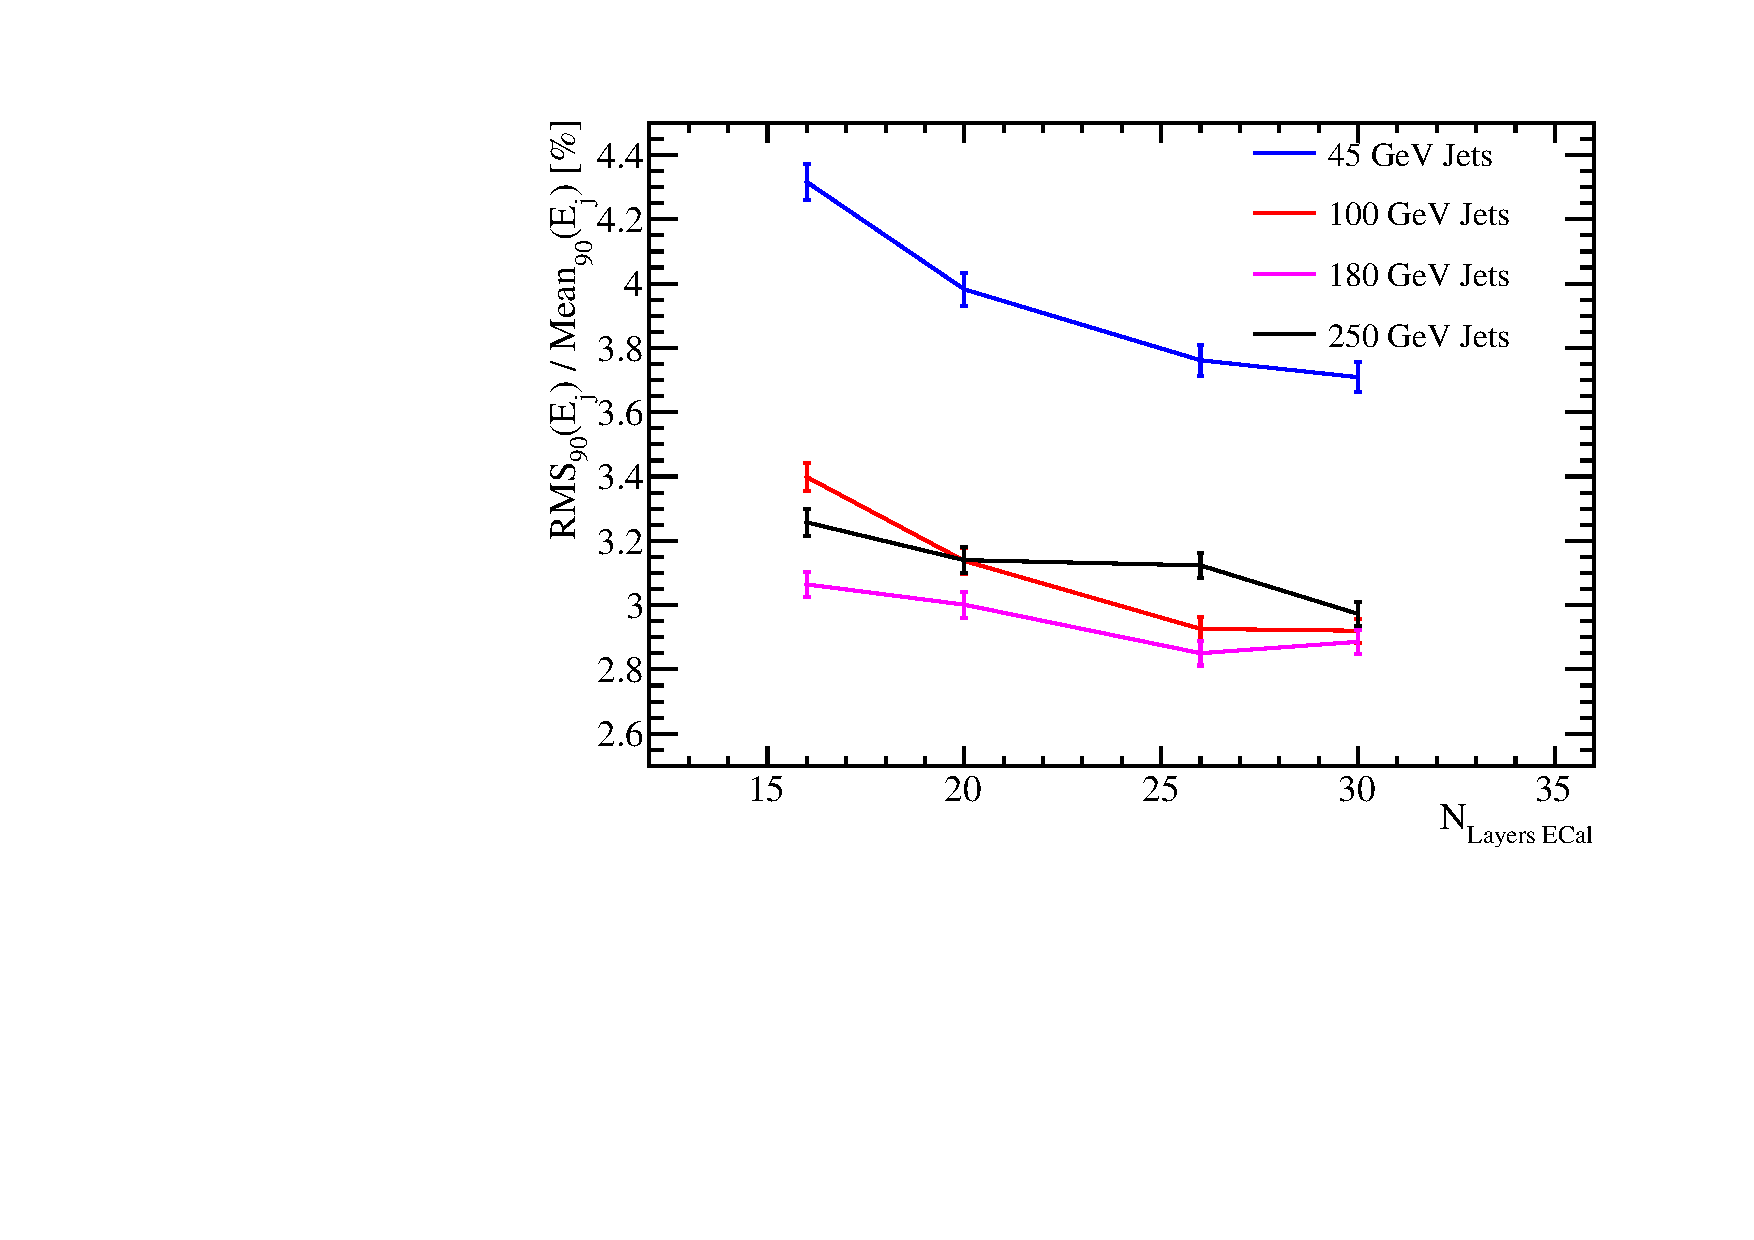
\includegraphics[width=0.5\textwidth]{OptimisationStudies/Plots/JetEnergyResolutions/JER_vs_SiliconECalNumberofLayers.pdf}}
\subfloat[Scintillator active material.]{\label{fig:ecalscnlayers}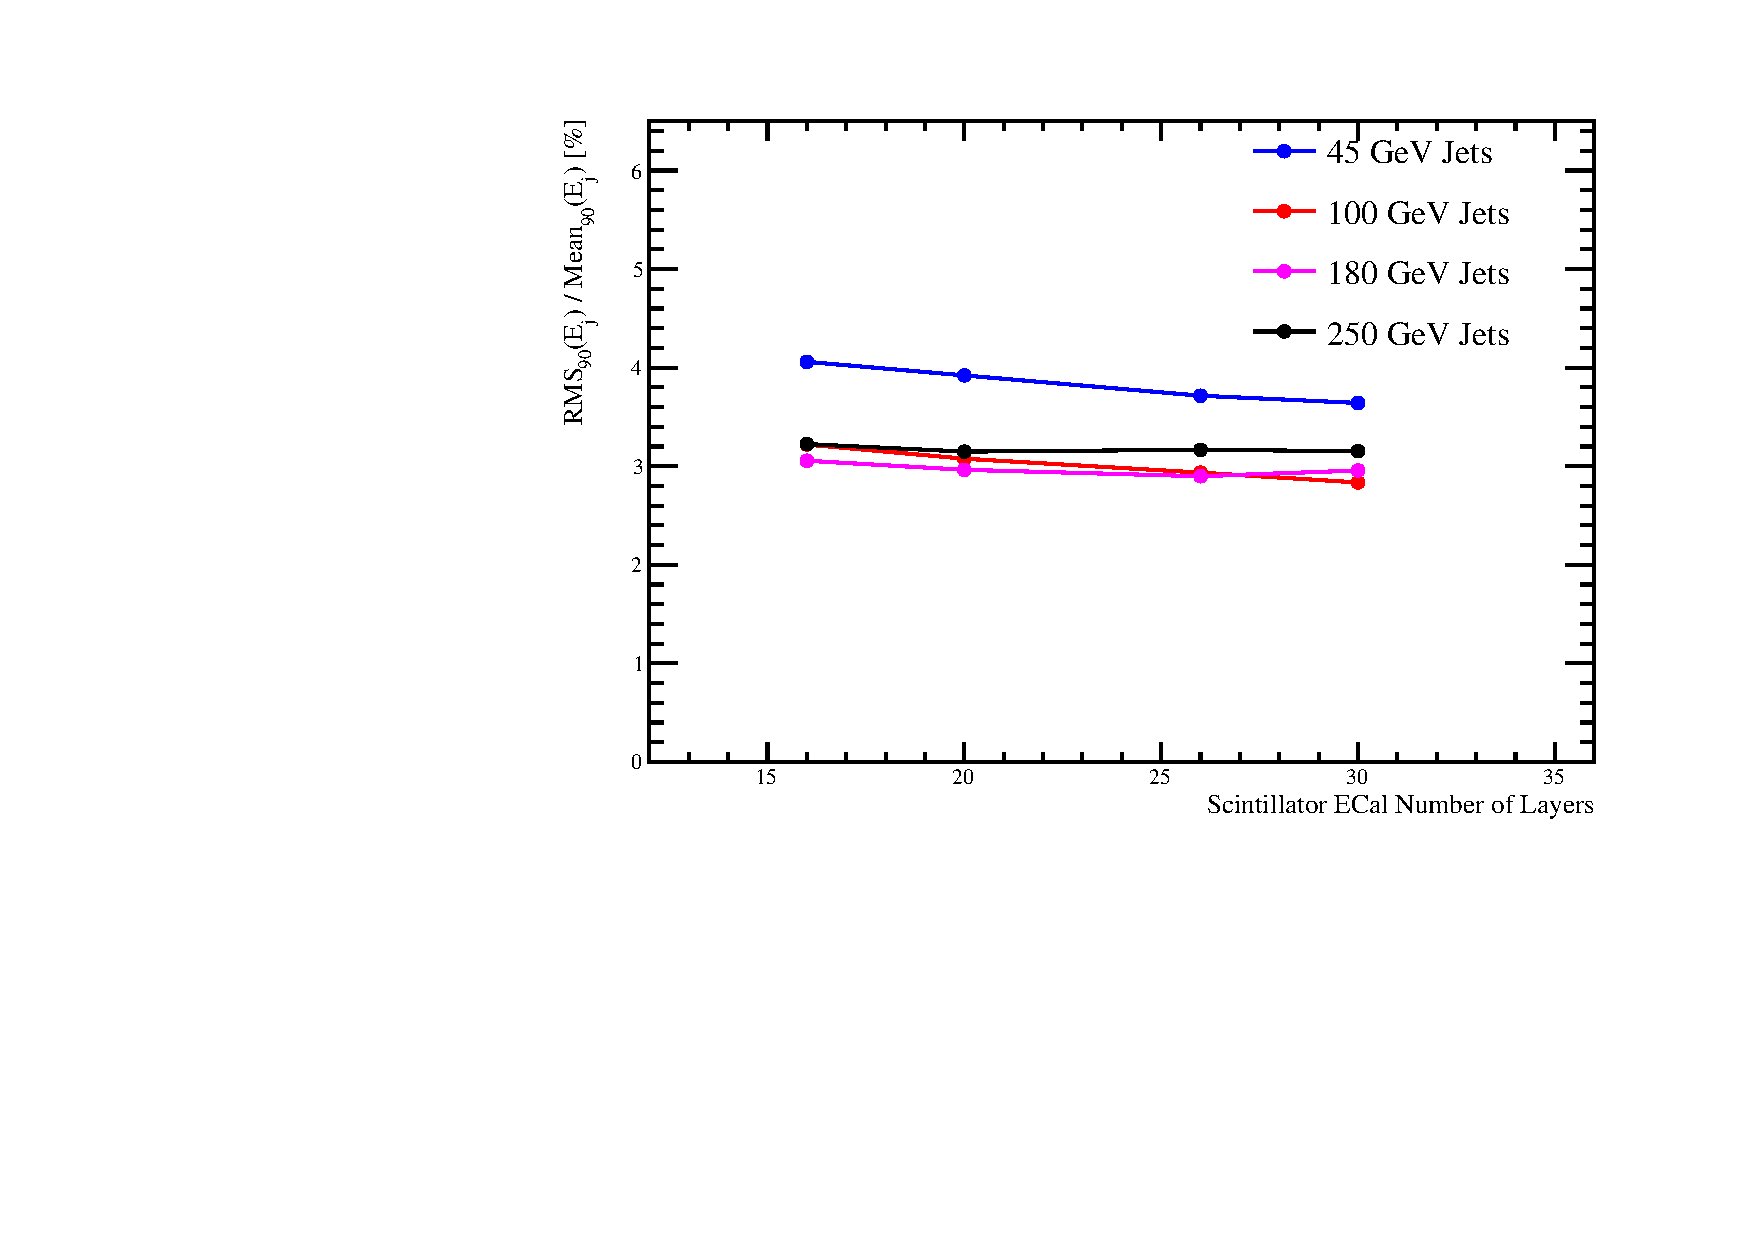
\includegraphics[width=0.5\textwidth]{OptimisationStudies/Plots/JetEnergyResolutions/JER_vs_ScintillatorECalNumberofLayers.pdf}} \hfill
\caption[Jet energy resolution as a function of longitudinal granularity in the ECal.]{Jet energy resolution as a function of longitudinal granularity in the ECal for the silicon and scintillator ECal options.}
\label{fig:ecalnlayers}
\end{figure}

The jet energy resolution was found to improve with increasing longitudinal granularity.  This is expected as a more layers in the calorimeter, for the same total thickness, implies greater sampling of the particle shower and so, as the energy resolution obeys Poissonian statistics, an improvement in the resolution.  

\begin{figure}
\centering
\subfloat[Silicon active material, 45 GeV Jets.]{\label{fig:ecalsinlayers45break}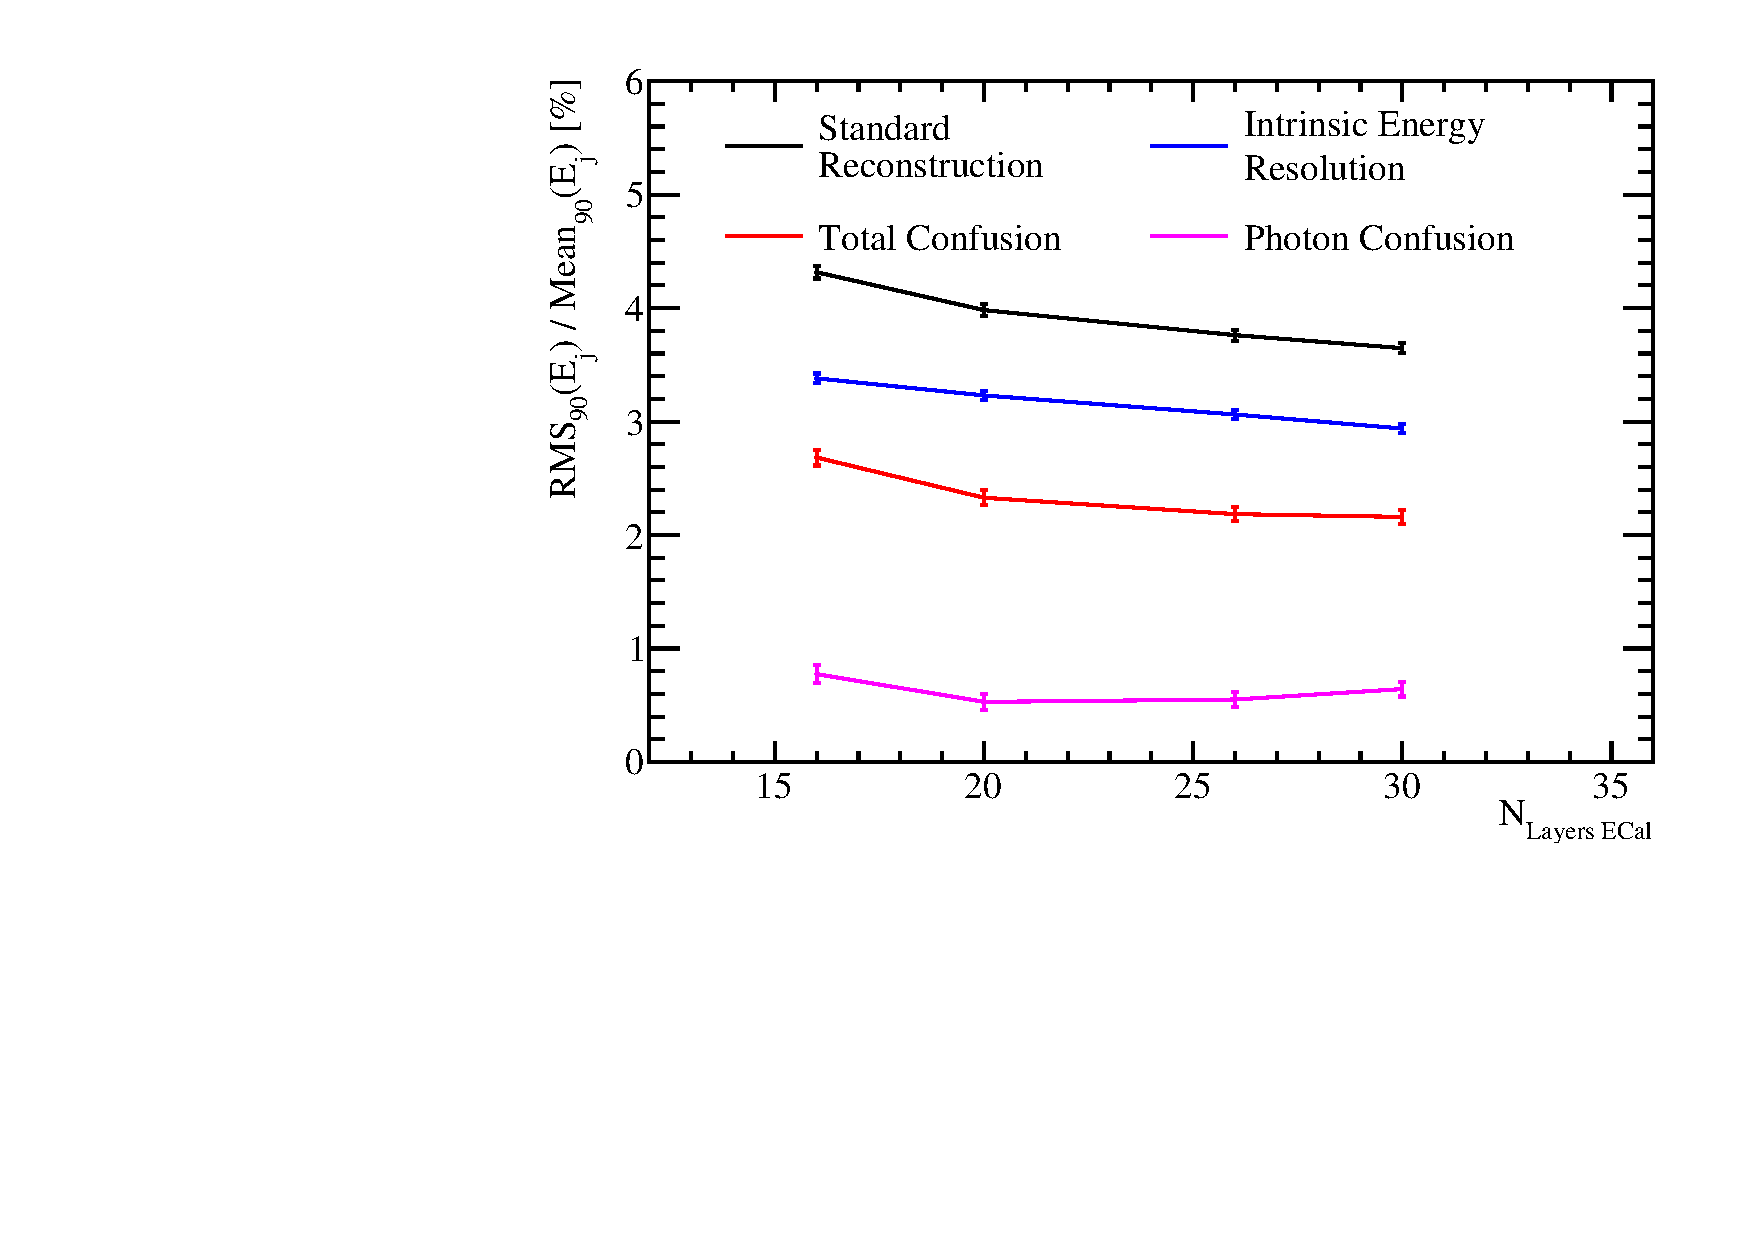
\includegraphics[width=0.5\textwidth]{OptimisationStudies/Plots/JetEnergyResolutions/JER_vs_SiliconECalNumberofLayers_91GeV_DiJet_Breakdown.pdf}}
\subfloat[Scintillator active material, 45 GeV Jets.]{\label{fig:ecalscnlayers45break}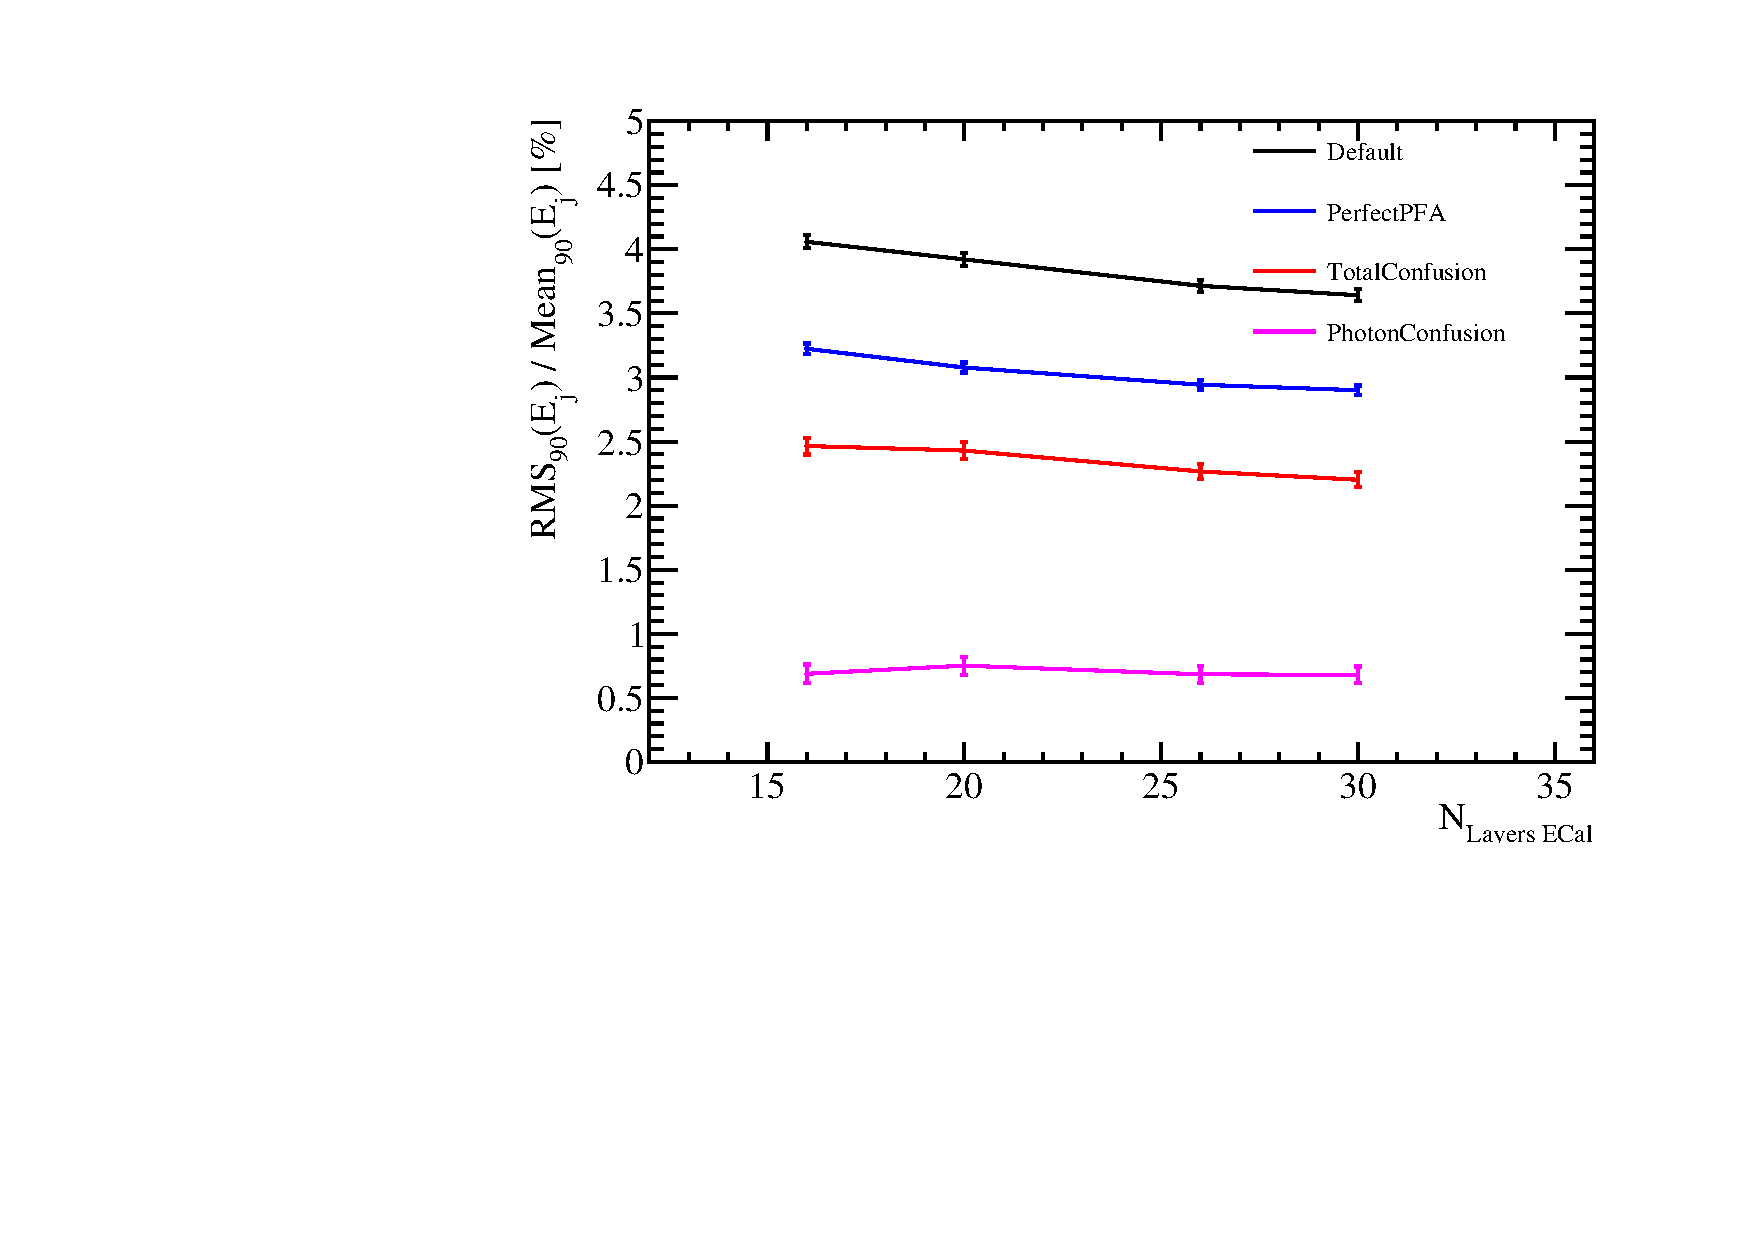
\includegraphics[width=0.5\textwidth]{OptimisationStudies/Plots/JetEnergyResolutions/JER_vs_ScintillatorECalNumberofLayers_91GeV_DiJet_Breakdown.pdf}} \hfill
\subfloat[Silicon active material, 250 GeV Jets.]{\label{fig:ecalsinlayers250break}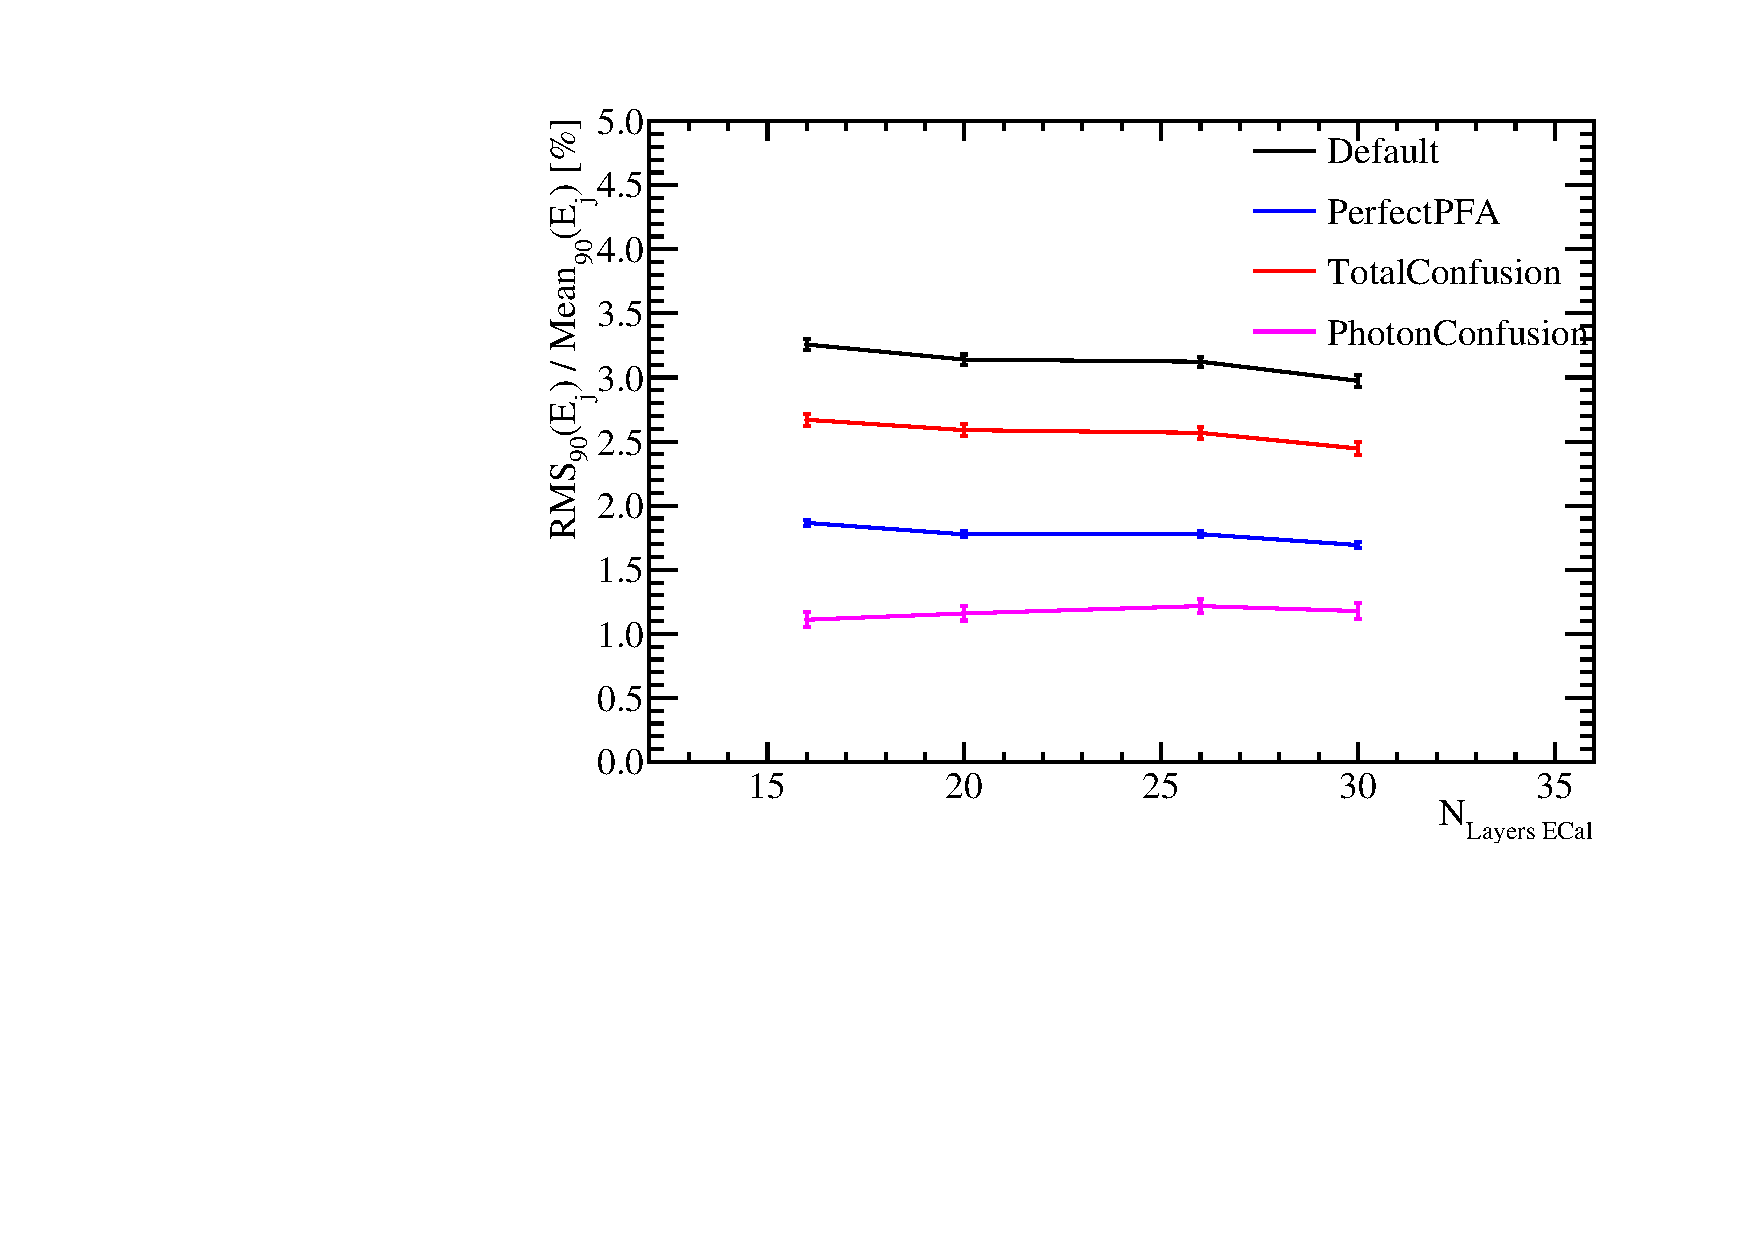
\includegraphics[width=0.5\textwidth]{OptimisationStudies/Plots/JetEnergyResolutions/JER_vs_SiliconECalNumberofLayers_500GeV_DiJet_Breakdown.pdf}}
\subfloat[Scintillator active material, 250 GeV Jets.]{\label{fig:ecalscnlayers250break}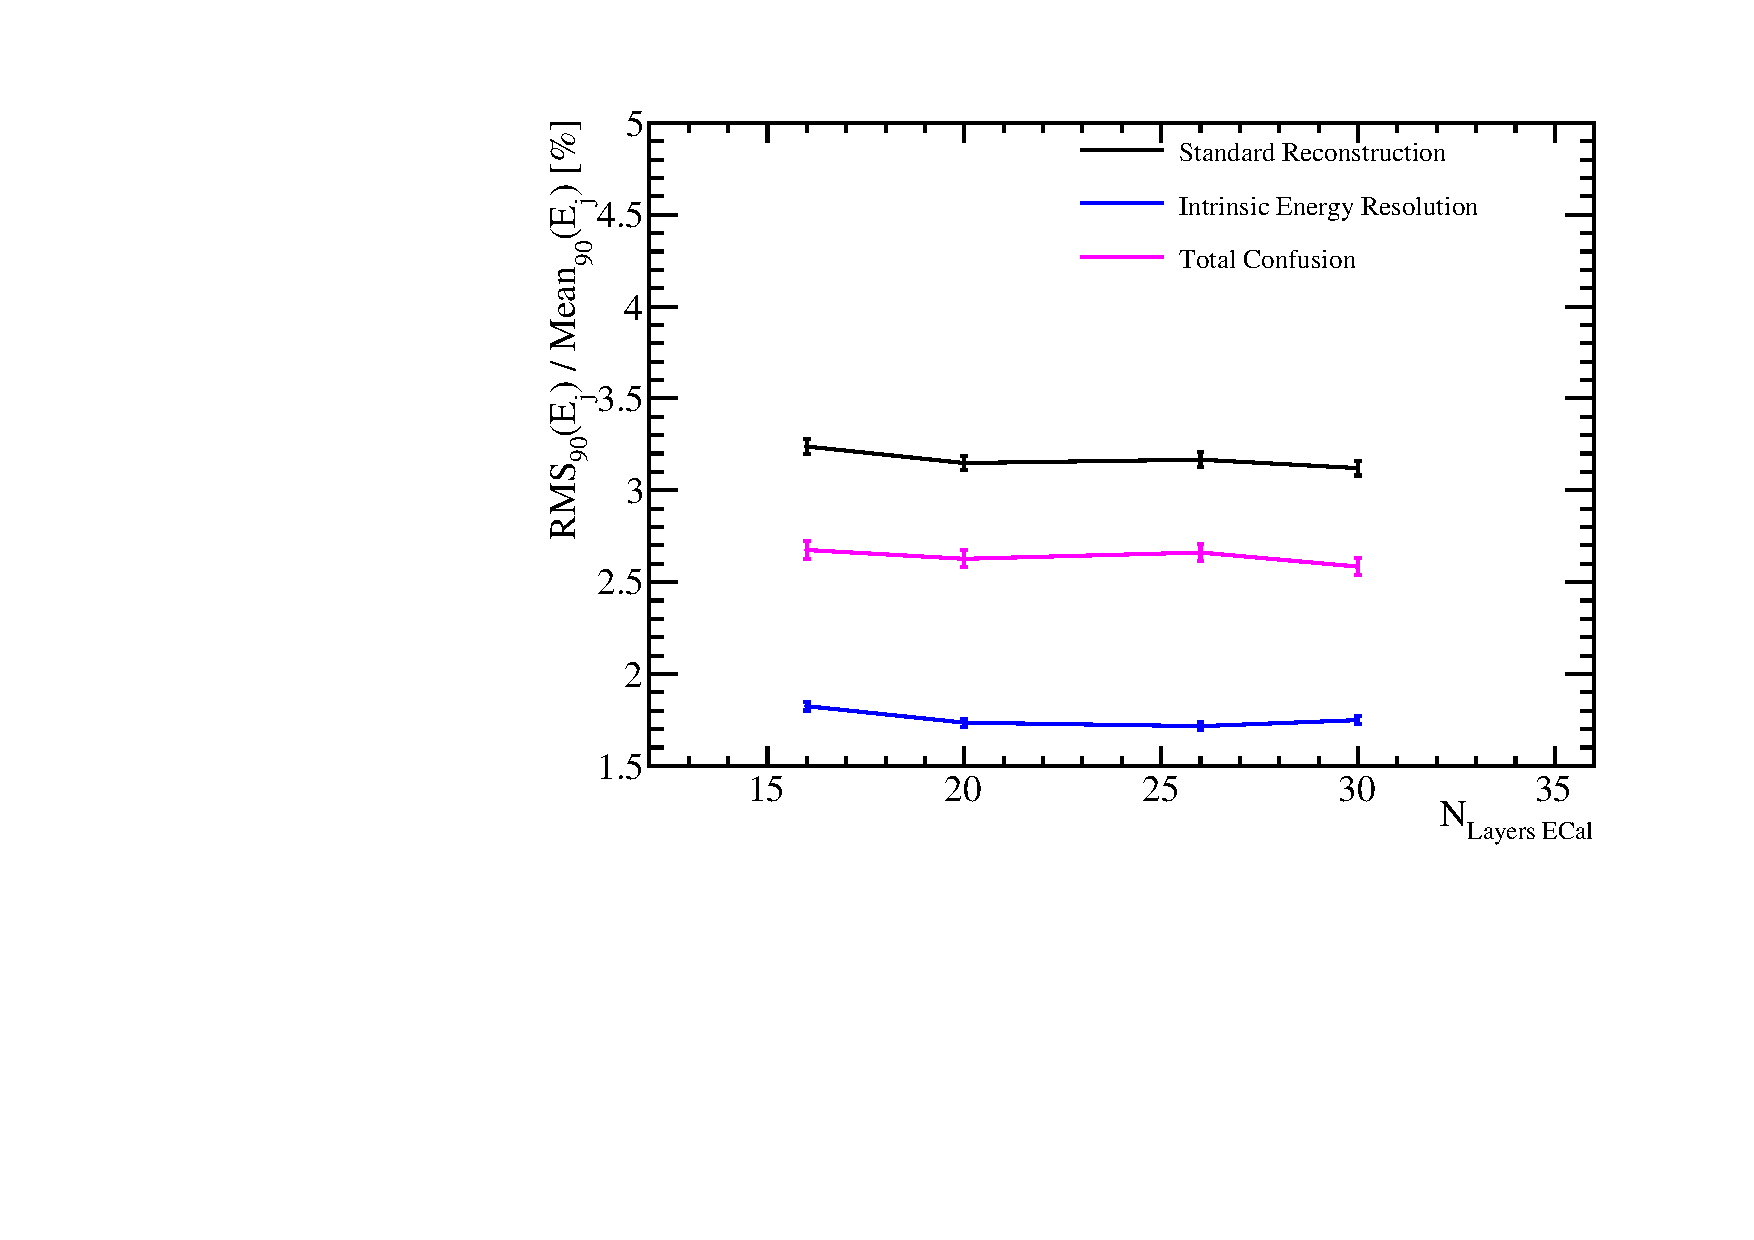
\includegraphics[width=0.5\textwidth]{OptimisationStudies/Plots/JetEnergyResolutions/JER_vs_ScintillatorECalNumberofLayers_500GeV_DiJet_Breakdown.pdf}}
\caption[Jet energy resolution breakdown as a function of ECal longitudinal granularity for 45 and 250 GeV jets.  Results are given for both the silicon and scintillator ECal options.]{Jet energy resolution breakdown as a function of ECal longitudinal granularity for 45 and 250 GeV jets.  Results are given for both the silicon and scintillator ECal options.}
\label{fig:ecalnlayers}
\end{figure}

When the jet energy resolution breakdowns as a function of ECal longitudinal granularity, figure \ref{fig:ecalnlayers}, are examined it becomes clear that the improvement to the resolution with finer longitudinal granularities occurs due to a twofold effect.  There is an improvement to the intrinsic energy resolution with more sampling of particle showers, while finer longitudinal granularity also reduces the impact of confusion.  In this case the reduction in confusion is not localised purely to the reconstruction of photons, as was largely the case for the ECal transverse granularity study, but extends to all reconstructed particles.  This indicates that finer longitudinal granularity in the ECal benefits the reconstruction of hadrons as well as photons and charged particles.







\iffalse

\section{Hadronic Calorimeter Optimsation}
\label{optstud:sec:hcal}

\subsection{HCal Transverse Granularity}
\label{optstud:sec:hcal:cellsize}

\begin{figure}
  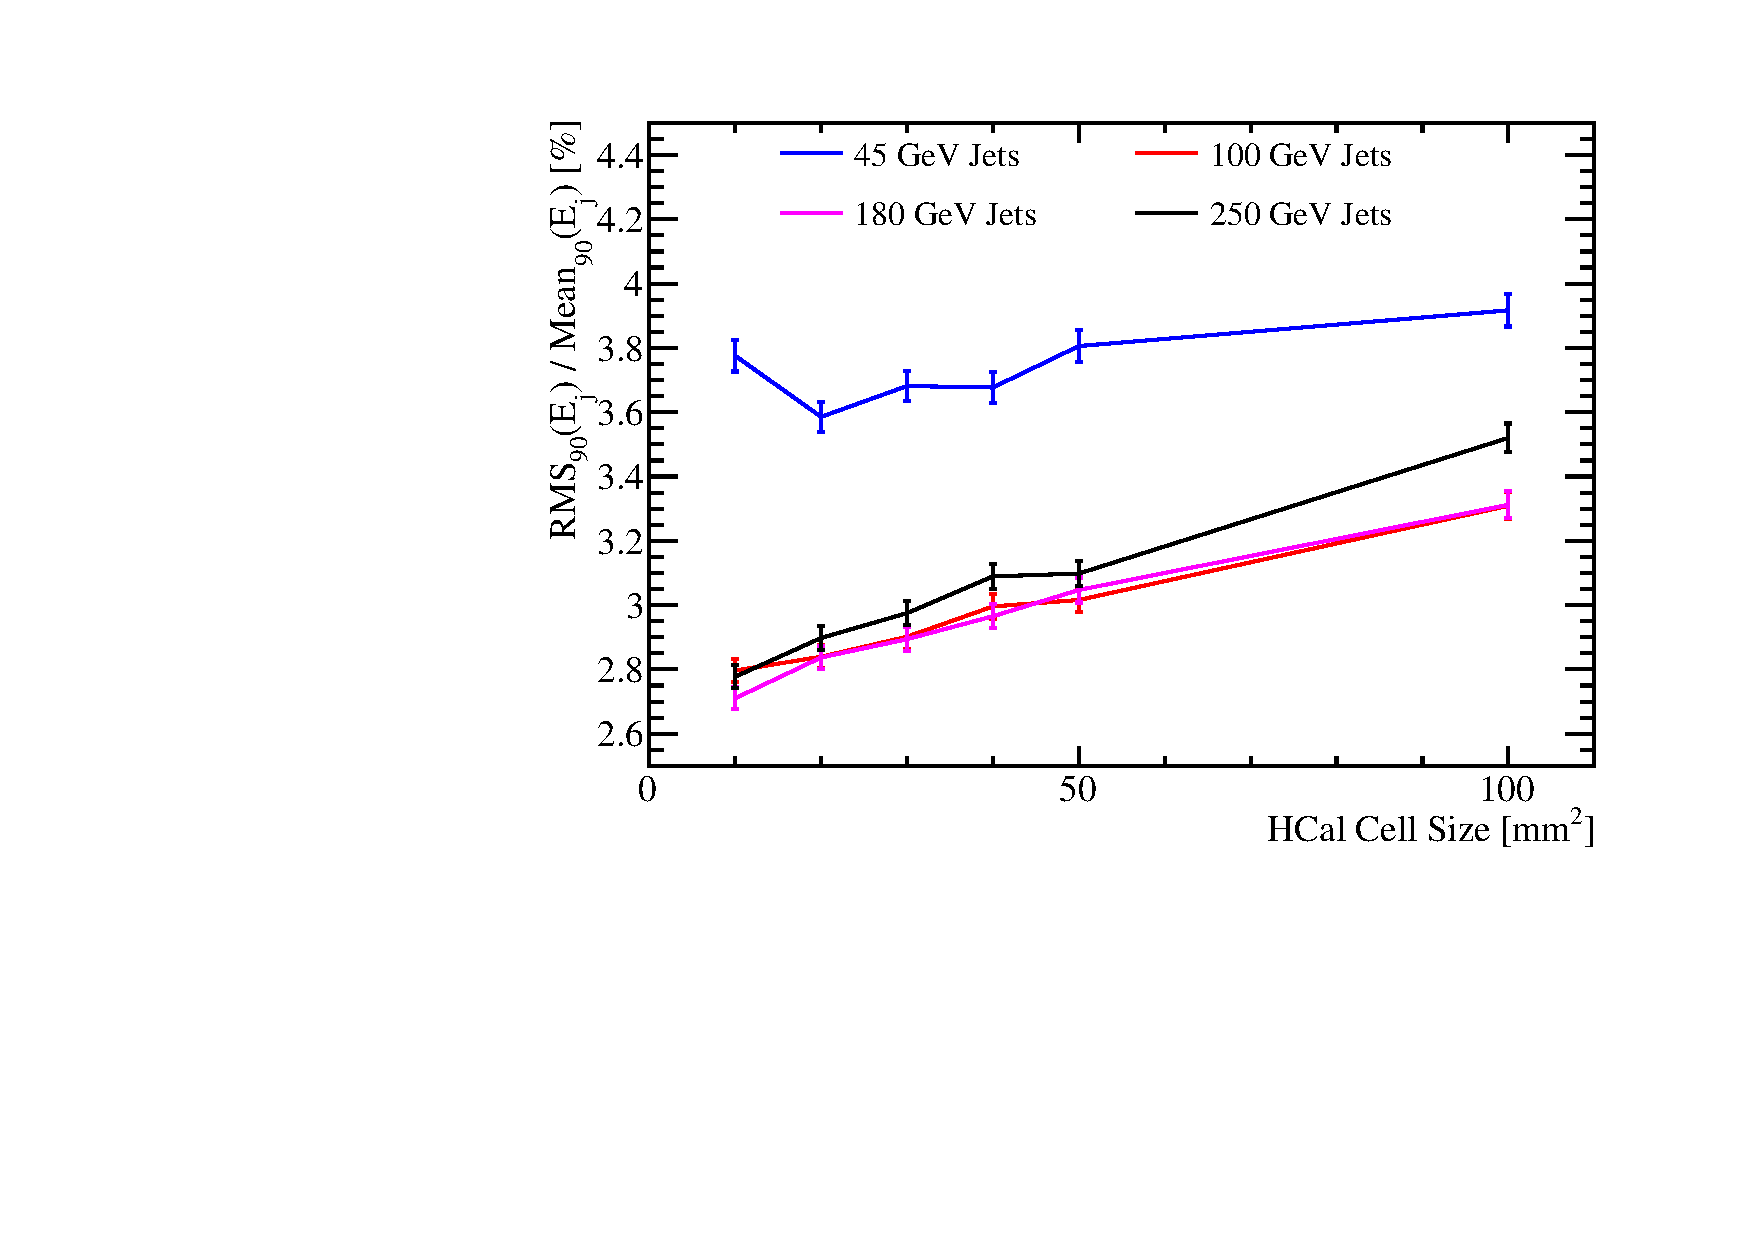
\includegraphics[width=0.5\textwidth]{OptimisationStudies/Plots/JetEnergyResolutions/JER_vs_HCalCellSize.pdf}
  \caption[Jet energy resolution as a function of HCal cell size for the scintillator steel HCal option.]{Jet energy resolution is shown for several fixed energy jets as a function of HCal cell size for the scintillator steel HCal option.}
  \label{optstud:fig:hcalcells}
\end{figure}

\subsection{HCal Longitudinal Granularity}
\label{optstud:sec:hcal:nlayers}

\begin{figure}
  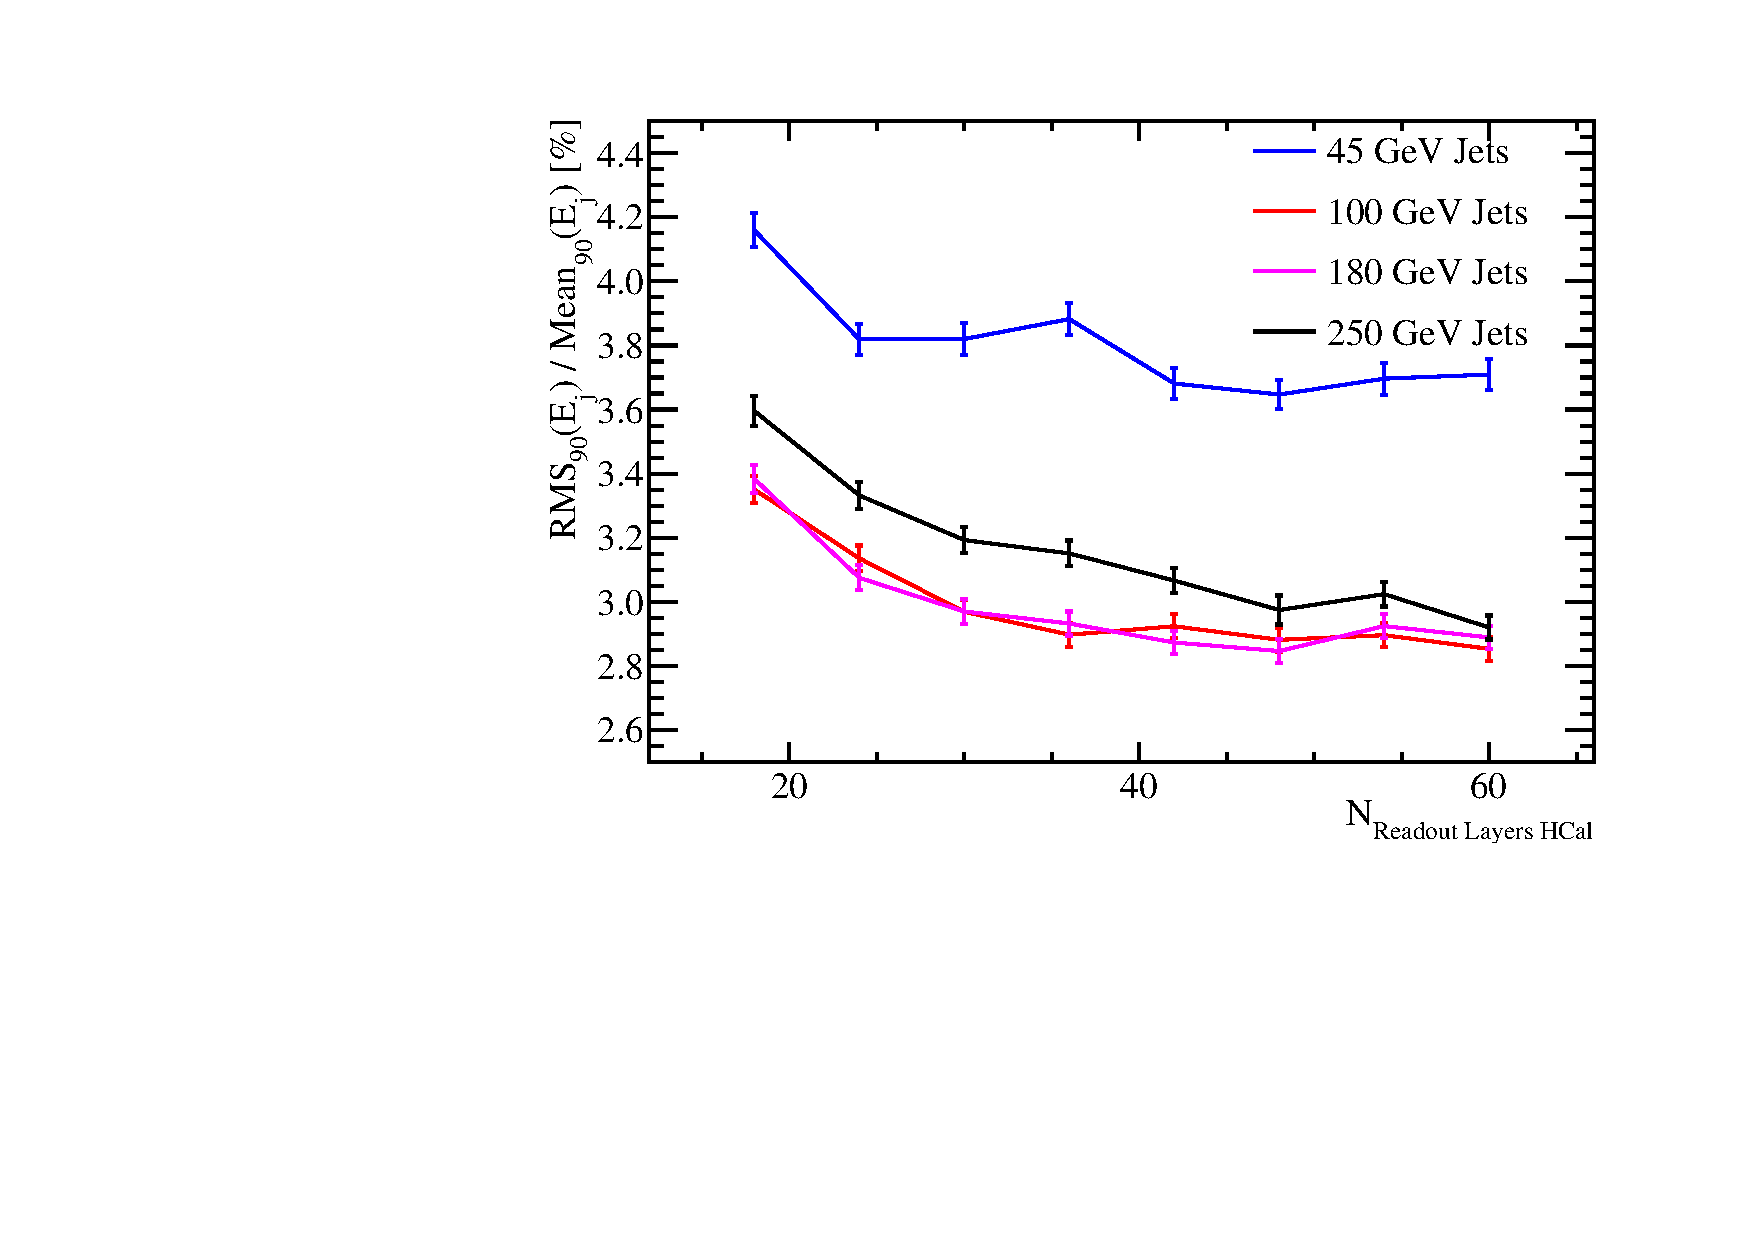
\includegraphics[width=0.5\textwidth]{OptimisationStudies/Plots/JetEnergyResolutions/JER_vs_NumberOfLayersInTheHCal.pdf}
  \caption[Jet energy resolution as a function of the number of layers in the HCal for the scintillator steel HCal option.]{Jet energy resolution is shown for several fixed energy jets as a function of the number of layers in the HCal for the scintillator steel HCal option.}
  \label{optstud:fig:hcalnlayers}
\end{figure}

\begin{figure}
  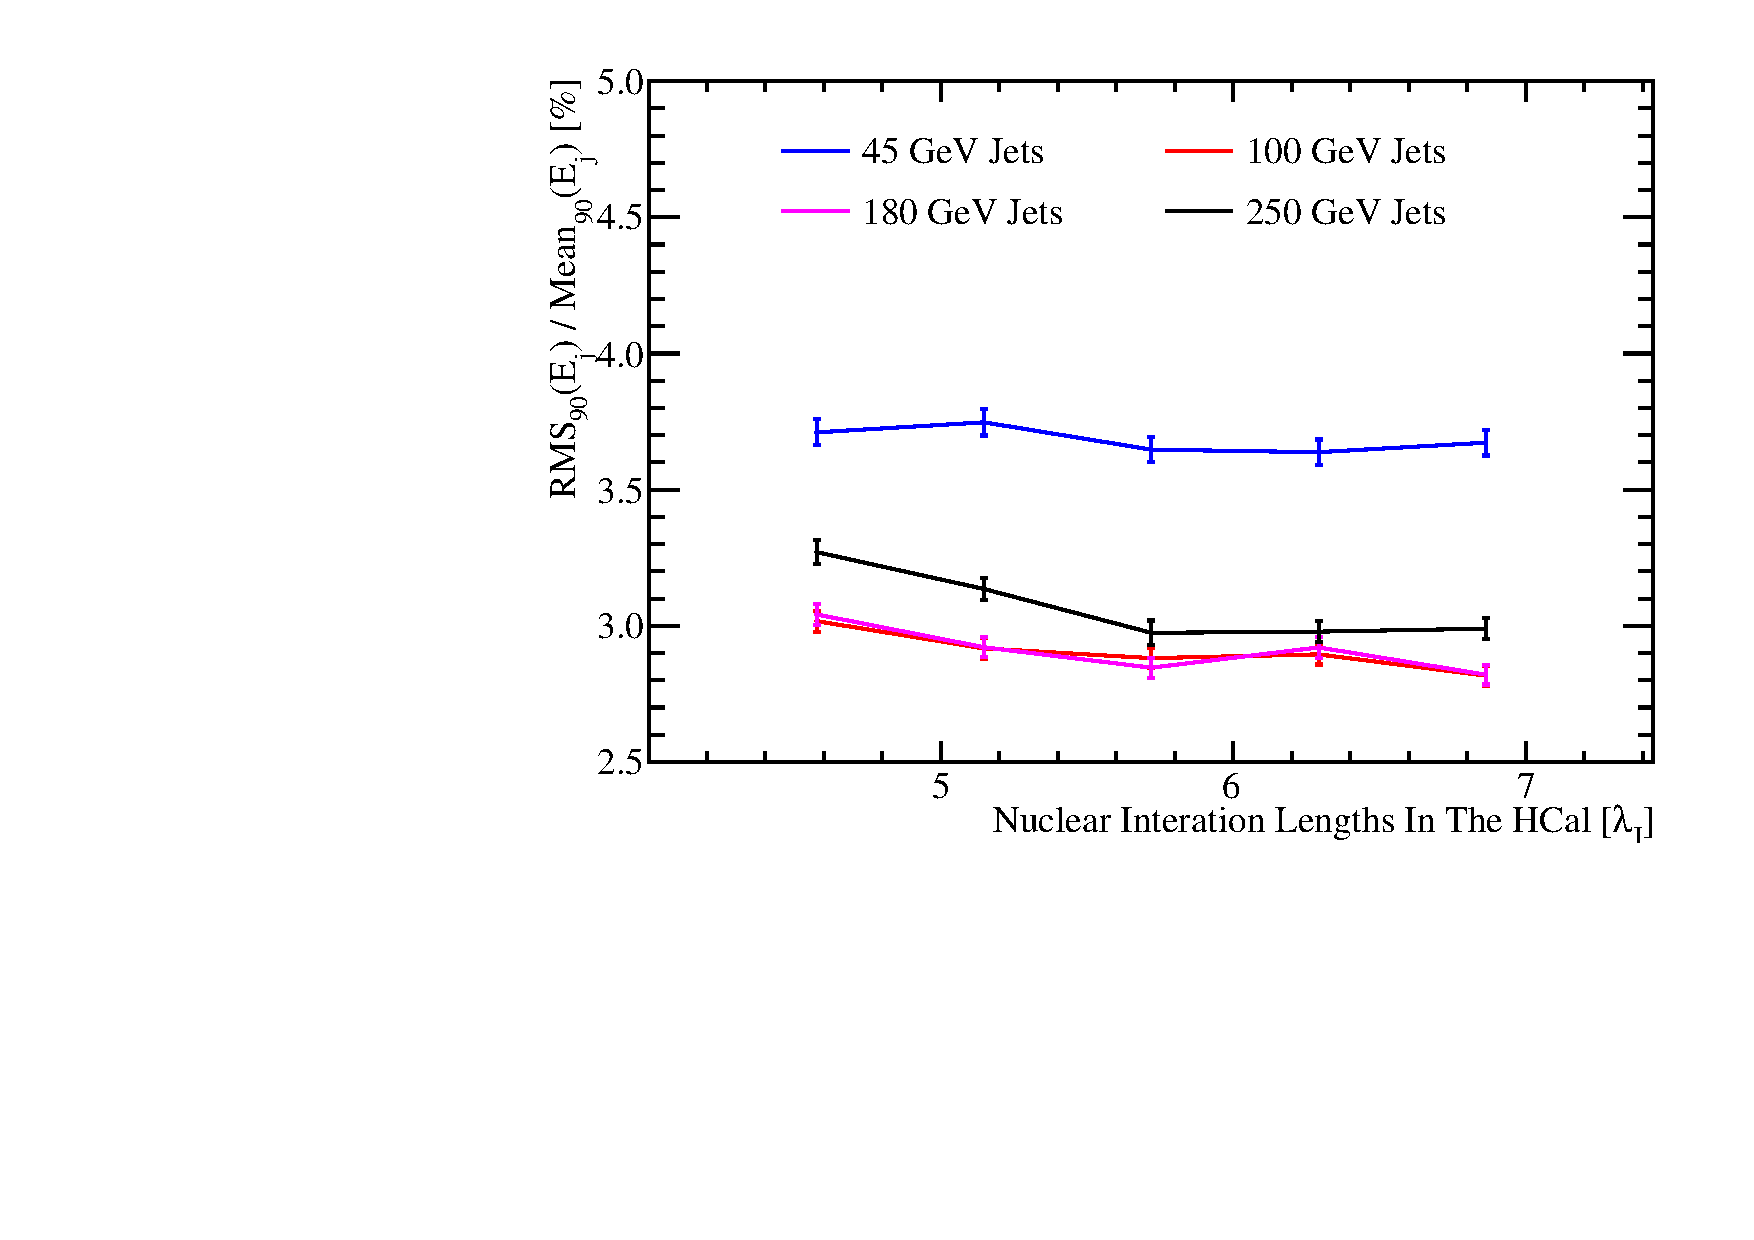
\includegraphics[width=0.5\textwidth]{OptimisationStudies/Plots/JetEnergyResolutions/JER_vs_NumberOfNuclearInterationLengthsInTheHCal.pdf}
  \caption[Jet energy resolution as a function of the number of nuclear interaction lengths in the HCal for the scintillator steel HCal option.]{Jet energy resolution is shown for several fixed energy jets as a function of the number of nuclear interation lenghts in the HCal for the scintillator steel HCal option.}
  \label{optstud:fig:hcaldepth}
\end{figure}

\begin{figure}
  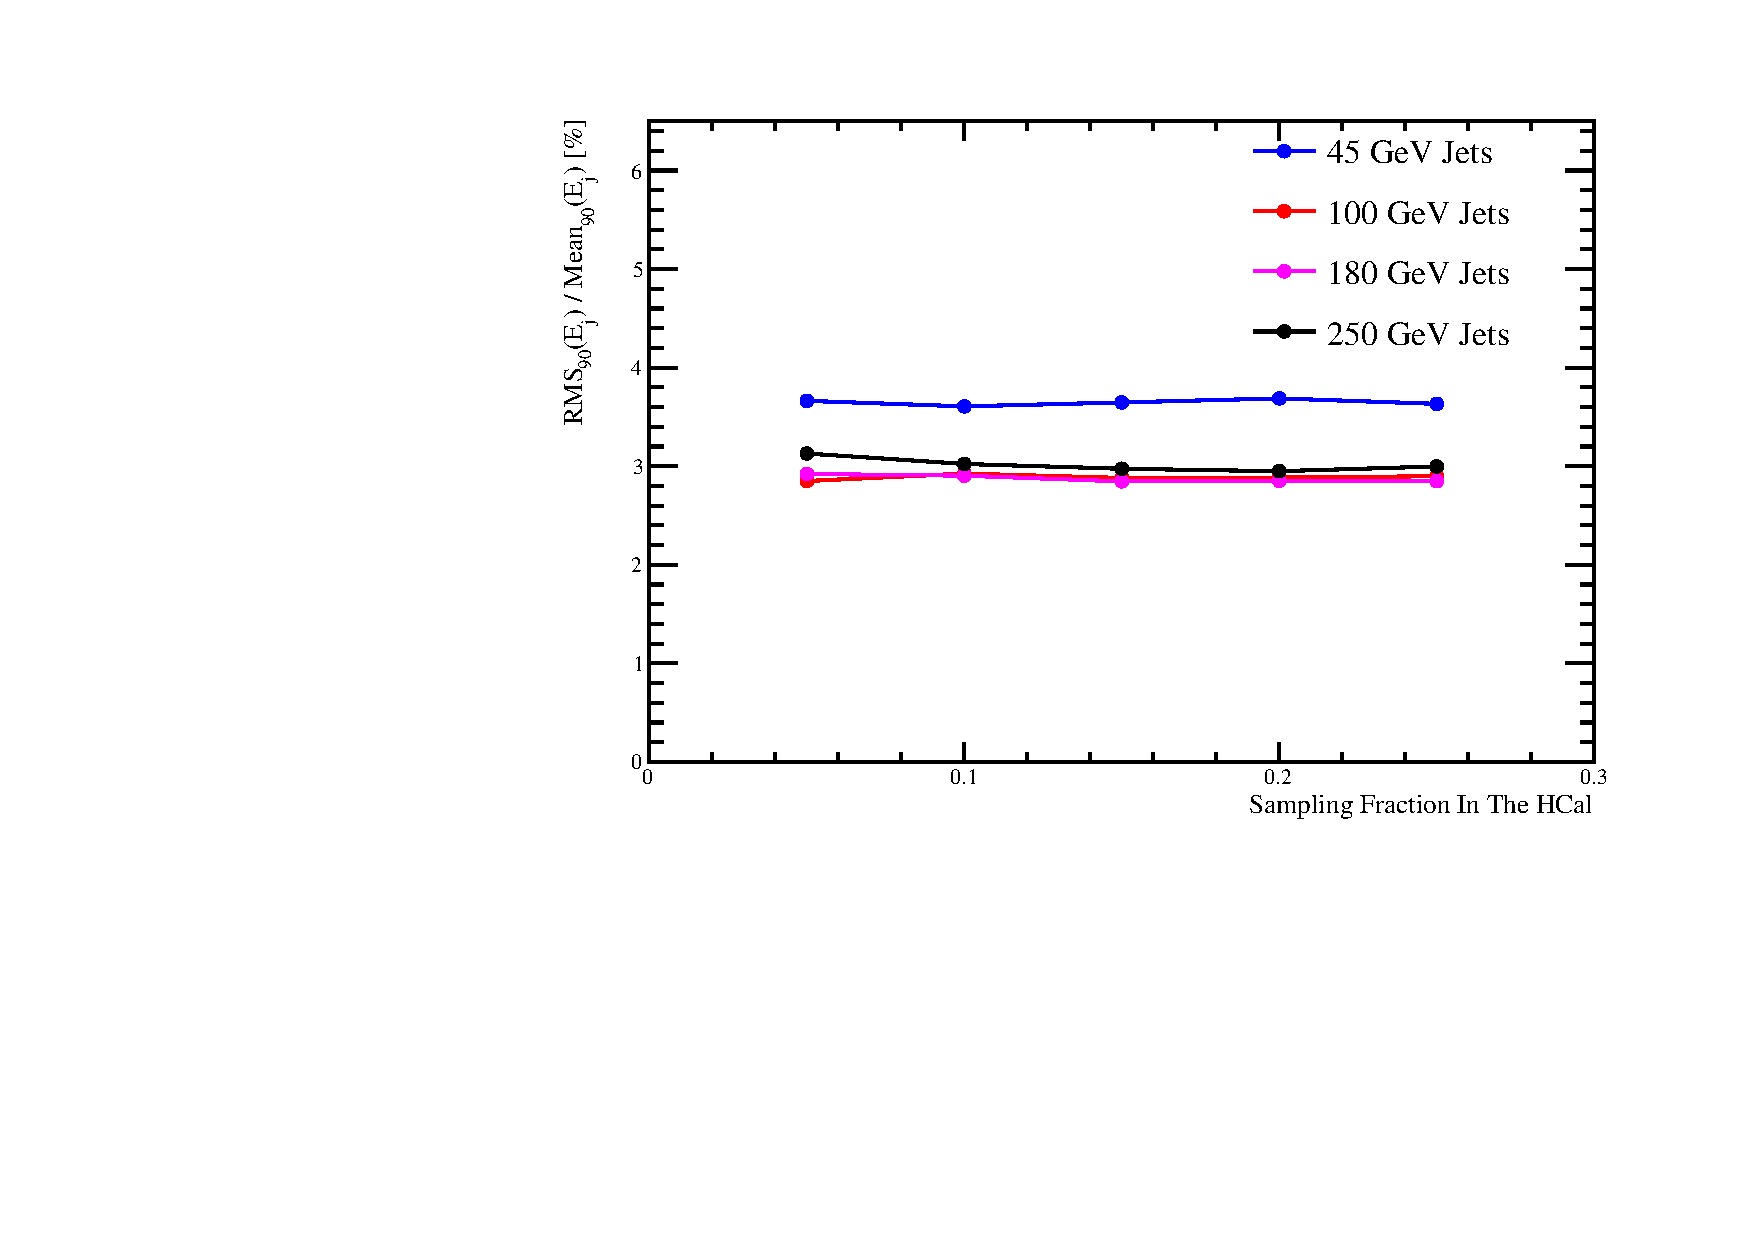
\includegraphics[width=0.5\textwidth]{OptimisationStudies/Plots/JetEnergyResolutions/JER_vs_SamplingFractionInTheHCal.pdf}
  \caption[Jet energy resolution as a function of the sampling fraction in the HCal for the scintillator steel HCal option.]{Jet energy resolution is shown for several fixed energy jets as a function of the sampling fraction in the HCal for the scintillator steel HCal option.}
  \label{optstud:fig:hcalsampfrac}
\end{figure}

\subsection{HCal Absorber Material}
\label{optstud:sec:hcal:absmat}

\begin{figure}
  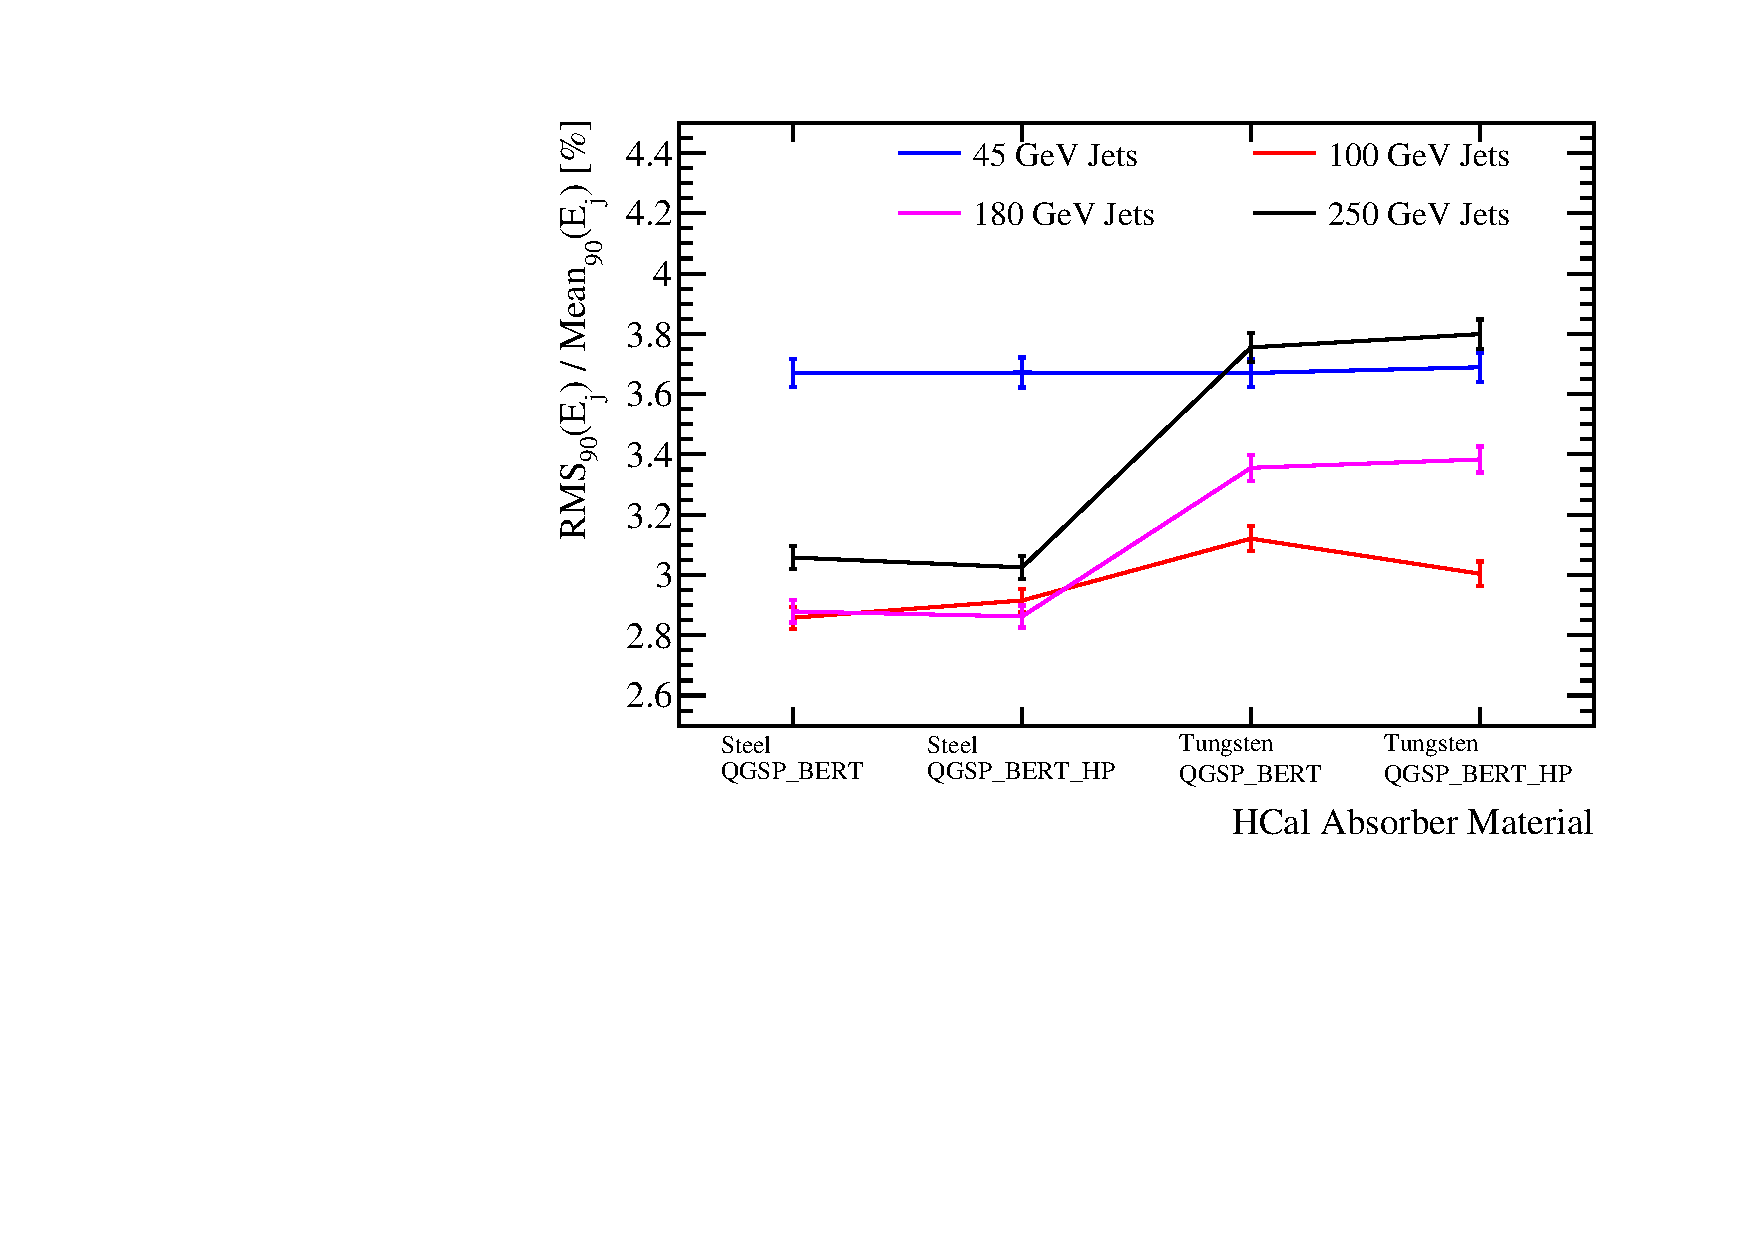
\includegraphics[width=0.5\textwidth]{OptimisationStudies/Plots/JetEnergyResolutions/JER_vs_HCalAbsorberMaterial.pdf}
  \caption[Jet energy resolution as a function of the absorber matieral in the HCal.]{Jet energy resolution is shown for several fixed energy jets as a function of the absorber material in the HCal.}
  \label{optstud:fig:hcalabsmat}
\end{figure}

\section{Global Detector Parameter Optimisation}
\label{optstud:sec:global}

\subsection{Magnetic Field Strength}
\label{optstud:sec:glob:bfield}

\begin{figure}
  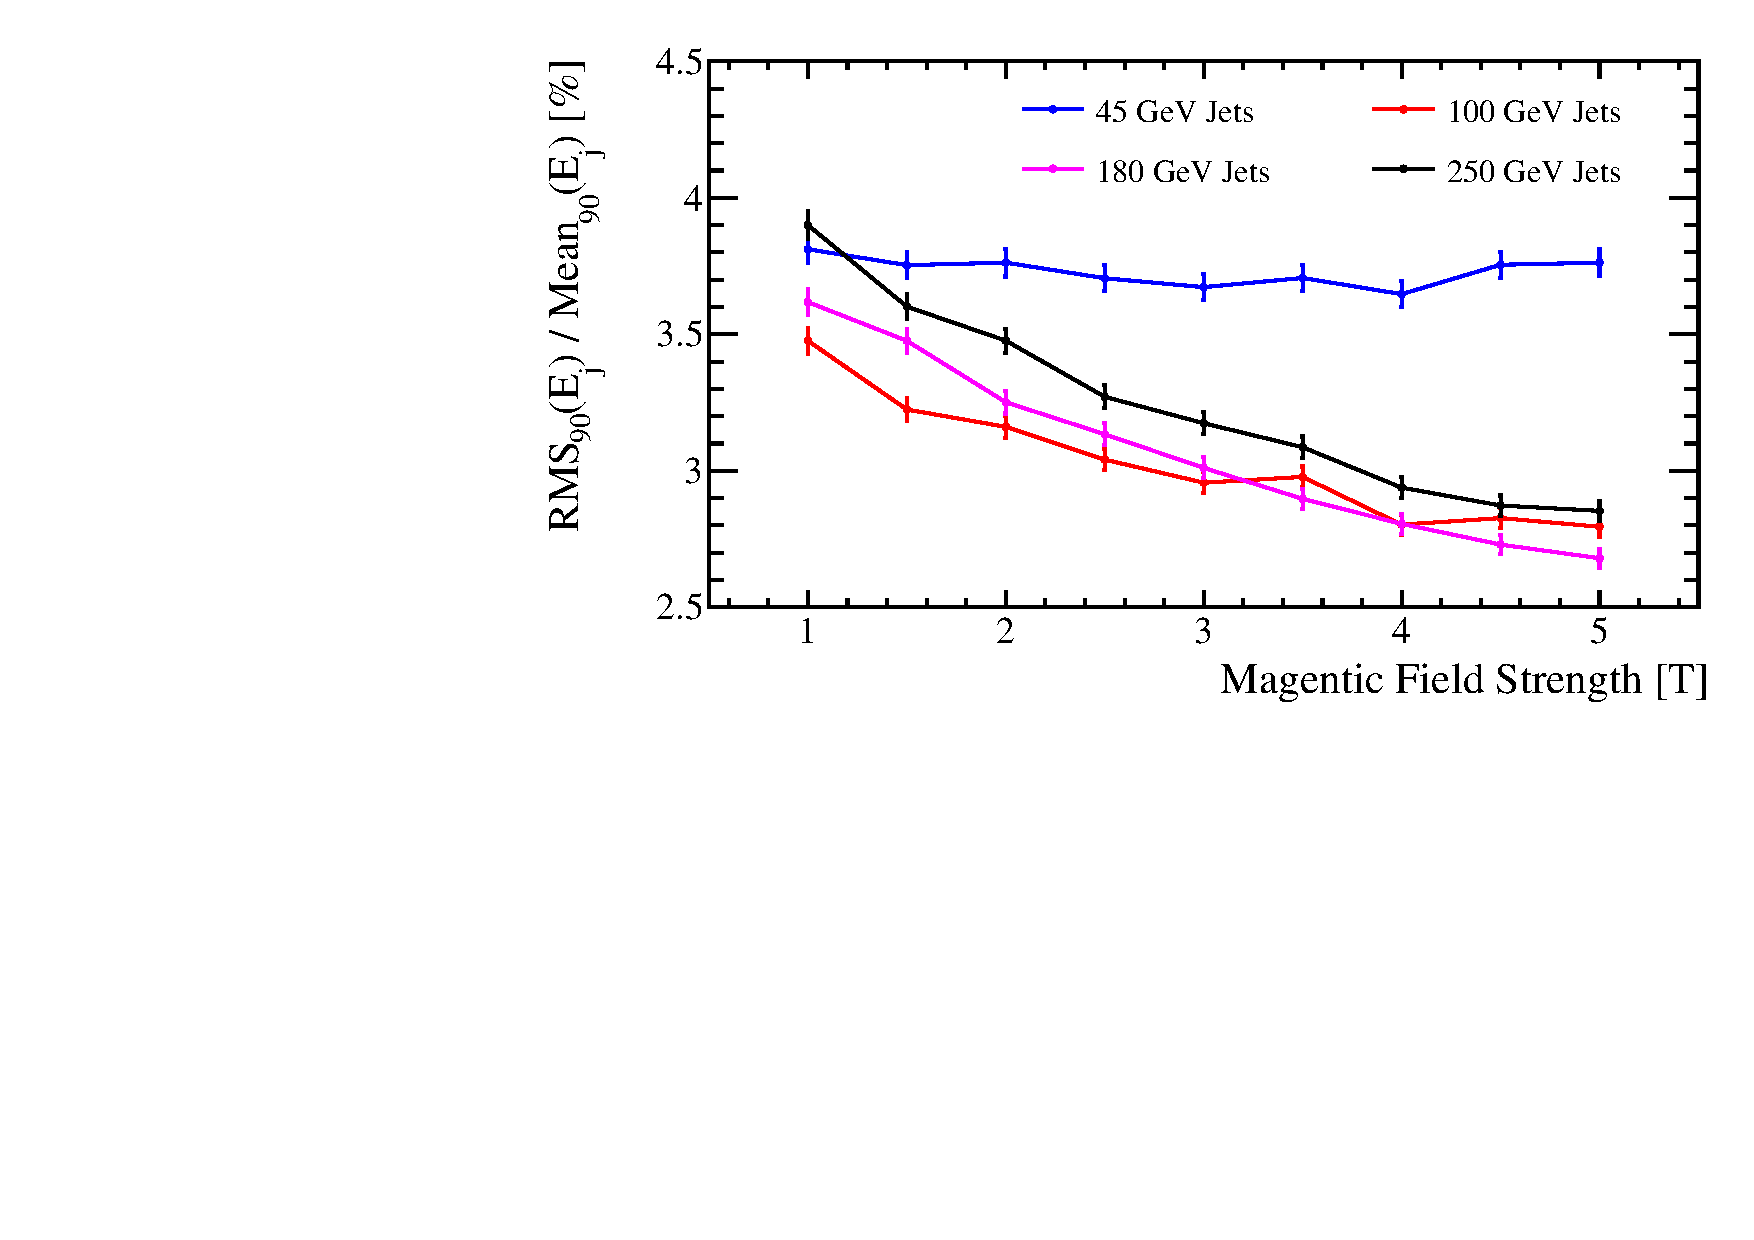
\includegraphics[width=0.5\textwidth]{OptimisationStudies/Plots/JetEnergyResolutions/JER_vs_MagneticField.pdf}
  \caption[Jet energy resolution as a function of magnetic field strength.]{Jet energy resolution is shown for several fixed energy jets as a function of magetic field strength.}
  \label{optstud:fig:bfield}
\end{figure}

\subsection{Inner ECal Radius}
\label{optstud:sec:glob:ecalinnerrad}

\begin{figure}
  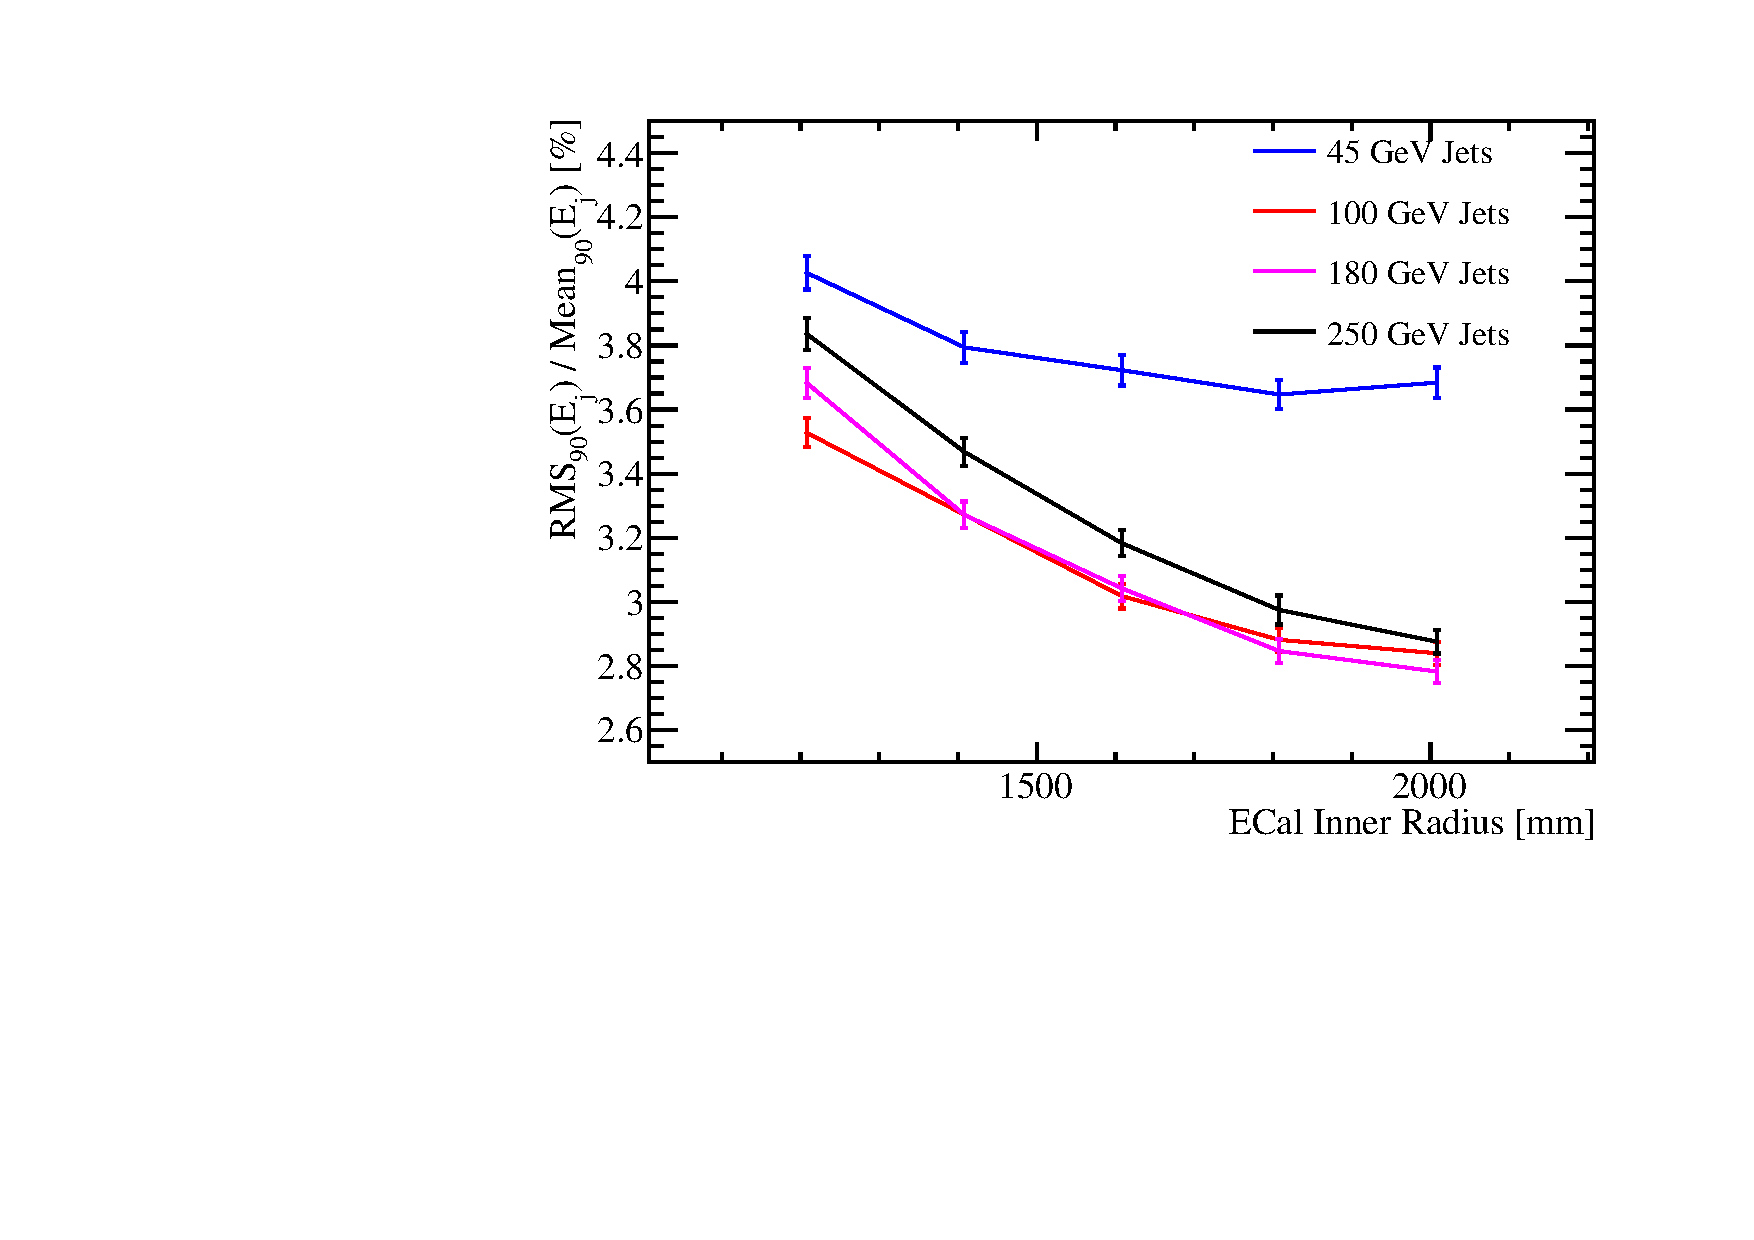
\includegraphics[width=0.5\textwidth]{OptimisationStudies/Plots/JetEnergyResolutions/JER_vs_ECalInnerRadius.pdf}
  \caption[Jet energy resolution as a function of the ECal inner radius.]{Jet energy resolution is shown for several fixed energy jets as a function of the inner ECal radius.}
  \label{optstud:fig:ecalinnerrad}
\end{figure}

\fi

\iffalse
JER_vs_BothECalCellSize.C                                   JER_vs_MagneticFieldStrength.C                              JER_vs_ScintillatorECalCellSize_91GeV_DiJet_Breakdown.pdf
JER_vs_BothECalNumberofLayers.C                             JER_vs_MagneticFieldStrength.pdf                            JER_vs_ScintillatorECalNumberofLayers.C
JER_vs_ECalInnerRadius.C                                    JER_vs_NumberOfLayersInTheHCal.C                            JER_vs_ScintillatorECalNumberofLayers.pdf
JER_vs_ECalInnerRadius.pdf                                  JER_vs_NumberOfLayersInTheHCal.pdf                          JER_vs_SiliconECalCellSize.C
JER_vs_HCalAbsorberMaterial.C                               JER_vs_NumberOfNuclearInterationLengthsInTheHCal.C          JER_vs_SiliconECalCellSize.pdf
JER_vs_HCalAbsorberMaterial.pdf                             JER_vs_NumberOfNuclearInterationLengthsInTheHCal.pdf        JER_vs_SiliconECalCellSize_500GeV_DiJet_Breakdown.C
JER_vs_HCalCellSize.C                                       JER_vs_SamplingFractionInTheHCal.C                          JER_vs_SiliconECalCellSize_500GeV_DiJet_Breakdown.pdf
JER_vs_HCalCellSize.pdf                                     JER_vs_SamplingFractionInTheHCal.pdf                        JER_vs_SiliconECalCellSize_91GeV_DiJet_Breakdown.C
JER_vs_HCalCellSize1000000GeVMHHHE.C                        JER_vs_ScintillatorECalCellSize.C                           JER_vs_SiliconECalCellSize_91GeV_DiJet_Breakdown.pdf
JER_vs_HCalCellSize1000000GeVMHHHE.pdf                      JER_vs_ScintillatorECalCellSize.pdf                         JER_vs_SiliconECalNumberofLayers.C
JER_vs_HCalCellSize1GeVMHHHE.C                              JER_vs_ScintillatorECalCellSize_500GeV_DiJet_Breakdown.C    JER_vs_SiliconECalNumberofLayers.pdf
JER_vs_HCalCellSize1GeVMHHHE.pdf                            JER_vs_ScintillatorECalCellSize_500GeV_DiJet_Breakdown.pdf  
JER_vs_MagneticField.pdf                                    JER_vs_ScintillatorECalCellSize_91GeV_DiJet_Breakdown.C 
\fi


